 %% Copyright (C) 2011, Andrea Cimino, All Rights Reserved.
 %% This file is distributed under the terms of the Creative Commons
 %% Licence Non-Commercial Share-Alike license

%% Useful stuff for separate compilation.
\ifx\ismaindoc\undefined
\providecommand{\inbpdocument}{
 \documentclass[11pt,a4paper,twoside,titlepage]{scrbook}
%%%%%%%%%%%%%%%%%%%%%%%%%%%%%%%%
%%%%%%%%%%% PACKAGES %%%%%%%%%%%
%%%%%%%%%%%%%%%%%%%%%%%%%%%%%%%%
% encoding
\usepackage[utf8x]{inputenc}
\usepackage[italian]{babel} % babel (suddivisione parole in sillabe)

\usepackage{amsfonts} % matematica
\usepackage{amsmath} % matematica
\usepackage{amssymb} % simboli vari
\usepackage{calrsfs}
\usepackage{caption}
\usepackage{enumerate}
\usepackage{extarrows} % matematica
\usepackage{keyval}
\usepackage{manfnt} % Simboli curva
\usepackage{mathtools} % matematica
\usepackage{multirow} 
\usepackage[usenames, dvipsnames]{color} % colori con nome
\usepackage[pdftex]{graphicx}
\usepackage{epstopdf} % gestione file EPS
\usepackage{wrapfig} % per figure circondate da testo
\usepackage{framed}	% teoremi framed
\usepackage{fancyhdr} % header buffi
\usepackage[T1]{fontenc} % gestione hbox e vbox
\usepackage[a4paper]{geometry}
\usepackage{microtype} % gestione hbox e vbox
\usepackage[thref, amsthm, amsmath, framed, hyperref]{ntheorem} % teoremi (avanzata)
%% \usepackage{prooftree} % gestione prof-tree
\usepackage{rotating}
\usepackage{stmaryrd}
\usepackage{subfig}
\usepackage{syntax} % syntattic stuff
\usepackage{txfonts}
\usepackage{verbatim} % migliorie al verbatim
%\usepackage{hyperref}
%% \usepackage{qtree}
\usepackage{fancyvrb}
\usepackage{listings}
\usepackage{cancel}
\usepackage{tikz}

\usepackage{bbding} %% Icons

%%%%%%%%%%%%%%%%%%%%%%%%%%%%%%%%
%%%%%%%%%%% GEOMETRY %%%%%%%%%%%
%%%%%%%%%%%%%%%%%%%%%%%%%%%%%%%%
\geometry{verbose,tmargin=2cm,bmargin=2.5cm,lmargin=2.5cm,rmargin=2cm}
\parindent0ex %% Remove paragraph indenting

%%%%%%%%%%%%%%%%%%%%%%%%%%%%%%%%
%%%%%%%%%%% CODE ENV %%%%%%%%%%%
%%%%%%%%%%%%%%%%%%%%%%%%%%%%%%%%
% codice
\newcounter{count}
\setcounter{count}{0}
\newenvironment{code}[1]
{
\color{lightgray}\hrulefill\color{code}
\stepcounter{count} {\bf\small Listato di codice \arabic{count}: {#1} }
\verbatim
}
{
\endverbatim
\color{lightgray}\hrulefill
\color{black}
\\
}

% codice semplice
\newenvironment{simplecode}
{
\color{code} \tt
}
{
\rm
}

 % Notation issues

%% Proof trees.
%\input prooftree
\newcommand*{\nohyp}{\phantom{x}}

%% C++.
\newcommand*{\Cplusplus}{{C\nolinebreak[4]\hspace{-.05em}\raisebox{.4ex}
{\tiny\bf ++}}}

%% BNF rules.
\newcommand*{\vbar}{\mathrel{\mid}}

%% Abstract syntax of the analyzed language.
\newcommand*{\Type}{\mathrm{Type}}
\newcommand*{\dType}{\mathrm{dType}}
\newcommand*{\dT}{\mathrm{dT}}
\newcommand*{\sType}{\mathrm{sType}}
\newcommand*{\sT}{\mathrm{sT}}
\newcommand*{\cType}{\mathrm{cType}}
\newcommand*{\cT}{\mathrm{cT}}
\newcommand*{\Integer}{\mathrm{Integer}}
\newcommand*{\Bool}{\mathrm{Bool}}
\newcommand*{\Id}{\mathrm{Id}}
\newcommand*{\id}{\mathrm{id}}
\newcommand*{\rId}{\mathrm{rId}}
\newcommand*{\idx}{\mathrm{x}}
\newcommand*{\ridx}{\underline{\mathrm{x}}}
\newcommand*{\Exp}{\mathrm{Exp}}
\newcommand*{\Exps}{\mathrm{Exps}}
\newcommand*{\Decl}{\mathrm{Decl}}
\newcommand*{\exceptDecl}{\mathrm{exceptDecl}}
\newcommand*{\Catch}{\mathrm{Catch}}
\newcommand*{\Stmt}{\mathrm{Stmt}}
\newcommand*{\Label}{\mathrm{Label}}
\newcommand*{\Con}{\mathrm{Con}}
\newcommand*{\con}{\mathrm{con}}
\newcommand*{\fps}{\mathrm{fps}}
\newcommand*{\funBody}{\mathrm{Body}}
\newcommand*{\funbody}{\mathrm{body}}
\newcommand*{\main}{\mathrm{main}}
\newcommand*{\es}{\mathrm{es}}
\newcommand*{\formParams}{\mathrm{formParams}}
\newcommand*{\emptysequence}{\boxempty}
\newcommand*{\Glob}{\mathrm{Glob}}

%% Sets of configurations
\newcommand*{\NTe}{\Gamma_\mathrm{e}}
\newcommand*{\NTb}{\Gamma_\mathrm{b}}
\newcommand*{\NTd}{\Gamma_\mathrm{d}}
\newcommand*{\NTg}{\Gamma_\mathrm{g}}
\newcommand*{\NTs}{\Gamma_\mathrm{s}}
\newcommand*{\NTk}{\Gamma_\mathrm{k}}
\newcommand*{\Te}{T_\mathrm{e}}
\newcommand*{\Tb}{T_\mathrm{b}}
\newcommand*{\Td}{T_\mathrm{d}}
\newcommand*{\Tg}{T_\mathrm{g}}
\newcommand*{\Ts}{T_\mathrm{s}}
\newcommand*{\Tk}{T_\mathrm{k}}

%% Lambda notation.
\newcommand*{\lambdaop}{\mathop{\lambda}\nolimits}

%% Sets of (no better specified) configurations.
\newcommand*{\NT}[1]{\Gamma_{#1}}
\newcommand*{\NTq}{\Gamma_q}
\newcommand*{\Tq}{T_q}

%% Denotable values.
\newcommand*{\dVal}{\mathrm{dVal}}
%% Storeable values.
\newcommand*{\sVal}{\mathrm{sVal}}
\newcommand*{\sval}{\mathrm{sval}}

%% Control modes.
\newcommand*{\CtrlMode}{\mathord{\mathrm{CtrlMode}}}
\newcommand*{\cm}{\mathrm{cm}}
%% Branch modes.
%\newcommand*{\BranchMode}{\mathord{\mathrm{BranchMode}}}
\newcommand*{\GotoMode}{\mathord{\mathrm{GotoMode}}}
\newcommand*{\SwitchMode}{\mathord{\mathrm{SwitchMode}}}
\newcommand*{\cmgoto}{\mathop{\mathrm{goto}}\nolimits}
\newcommand*{\cmswitch}{\mathop{\mathrm{switch}}\nolimits}
\newcommand*{\cmbreak}{\mathop{\mathrm{break}}\nolimits}
\newcommand*{\cmcontinue}{\mathop{\mathrm{continue}}\nolimits}
\newcommand*{\cmreturn}{\mathop{\mathrm{return}}\nolimits}
%% Exec mode.
\newcommand*{\cmexec}{\mathrm{exec}}
%% Value mode.
\newcommand*{\ValMode}{\mathord{\mathrm{ValMode}}}
\newcommand*{\cmvalue}{\mathop{\mathrm{value}}\nolimits}
%% Environment mode.
\newcommand*{\EnvMode}{\mathord{\mathrm{EnvMode}}}
\newcommand*{\cmenv}{\mathrm{env}}
%% Exception modes.
\newcommand*{\ExceptMode}{\mathord{\mathrm{ExceptMode}}}
\newcommand*{\cmexcept}{\mathrm{except}}

%% Control states.
\newcommand*{\CtrlState}{\mathord{\mathrm{CtrlState}}}
\newcommand*{\cs}{\mathord{\mathrm{cs}}}
%% Value states.
\newcommand*{\ValState}{\mathord{\mathrm{ValState}}}
\newcommand*{\valstate}{\upsilon}
%% Environment states.
%\newcommand*{\EnvState}{\mathord{\mathrm{EnvState}}}
%% Exception states.
\newcommand*{\ExceptState}{\mathord{\mathrm{ExceptState}}}
\newcommand*{\exceptstate}{\varepsilon}

%% Keywords.
\newcommand*{\kw}[1]{\mathop{\textup{\textbf{#1}}}}

\newcommand*{\bop}{\mathbin{\mathrm{bop}}}
%\newcommand*{\uop}{\mathop{\mathrm{uop}}}

%% Things that hold by definition.
\newcommand{\defrel}[1]{\mathrel{\buildrel \mathrm{def} \over {#1}}}
\newcommand{\defeq}{\defrel{=}}
\newcommand{\defiff}{\defrel{\Longleftrightarrow}}
%\newcommand{\defeq}{=}
%\newcommand{\defiff}{\Longleftrightarrow}

%% Divergence relation
\newcommand{\diverges}{\,\mathord{\buildrel \infty \over \longrightarrow}}

%% Special letters denoting sets and algebras.
\providecommand*{\Nset}{\mathbb{N}}             % Naturals
\providecommand*{\Qset}{\mathbb{Q}}             % Rationals
\providecommand*{\Zset}{\mathbb{Z}}             % Integers
\providecommand*{\Rset}{\mathbb{R}}             % Reals

%% Calligraphic alphabet.
\newcommand*{\calA}{\ensuremath{\mathcal{A}}}
\newcommand*{\calB}{\ensuremath{\mathcal{B}}}
\newcommand*{\calC}{\ensuremath{\mathcal{C}}}
\newcommand*{\calD}{\ensuremath{\mathcal{D}}}
\newcommand*{\calE}{\ensuremath{\mathcal{E}}}
\newcommand*{\calF}{\ensuremath{\mathcal{F}}}
\newcommand*{\calG}{\ensuremath{\mathcal{G}}}
\newcommand*{\calH}{\ensuremath{\mathcal{H}}}
\newcommand*{\calI}{\ensuremath{\mathcal{I}}}
\newcommand*{\calJ}{\ensuremath{\mathcal{J}}}
\newcommand*{\calK}{\ensuremath{\mathcal{K}}}
\newcommand*{\calL}{\ensuremath{\mathcal{L}}}
\newcommand*{\calM}{\ensuremath{\mathcal{M}}}
\newcommand*{\calN}{\ensuremath{\mathcal{N}}}
\newcommand*{\calO}{\ensuremath{\mathcal{O}}}
\newcommand*{\calP}{\ensuremath{\mathcal{P}}}
\newcommand*{\calQ}{\ensuremath{\mathcal{Q}}}
\newcommand*{\calR}{\ensuremath{\mathcal{R}}}
\newcommand*{\calS}{\ensuremath{\mathcal{S}}}
\newcommand*{\calT}{\ensuremath{\mathcal{T}}}
\newcommand*{\calU}{\ensuremath{\mathcal{U}}}
\newcommand*{\calV}{\ensuremath{\mathcal{V}}}
\newcommand*{\calW}{\ensuremath{\mathcal{W}}}
\newcommand*{\calX}{\ensuremath{\mathcal{X}}}
\newcommand*{\calY}{\ensuremath{\mathcal{Y}}}
\newcommand*{\calZ}{\ensuremath{\mathcal{Z}}}

%% Declarators for functions and relations.
\newcommand*{\reld}[3]{\mathord{#1}\subseteq#2\times#3}
\newcommand*{\fund}[3]{\mathord{#1}\colon#2\to#3}
\newcommand*{\pard}[3]{\mathord{#1}\colon#2\rightarrowtail#3}

%% Logical quantifiers stuff.
\newcommand{\st}{\mathrel{.}}
\newcommand{\itc}{\mathrel{:}}

%% Domain, codomain and range of a function.
\newcommand*{\dom}{\mathop{\mathrm{dom}}\nolimits}
%\newcommand*{\cod}{\mathop{\mathrm{cod}}\nolimits}
%\newcommand*{\range}{\mathop{\mathrm{range}}\nolimits}

%% Restriction of a function.
\newcommand*{\restrict}[1]{\mathop{\mid}\nolimits_{#1}}

%% Type of a constant.
\newcommand*{\type}{\mathop{\mathrm{type}}\nolimits}

%% Lubs, glbs, and fixed points.
\newcommand*{\lub}{\mathop{\mathrm{lub}}\nolimits}
%\newcommand*{\glb}{\mathop{\mathrm{glb}}\nolimits}
\newcommand*{\lfp}{\mathop{\mathrm{lfp}}\nolimits}
\newcommand*{\gfp}{\mathop{\mathrm{gfp}}\nolimits}

%% Generic widening.
\newcommand*{\widen}{\mathbin{\nabla}}

%% Set theory.
\renewcommand{\emptyset}{\varnothing}

%\newcommand*{\wpc}{\mathop{\wp_\mathrm{c}}\nolimits}
%\newcommand*{\wpf}{\mathop{\wp_\mathrm{f}}\nolimits}
%\newcommand*{\wpn}{\mathop{\wp_\mathrm{n}}\nolimits}

\newcommand*{\sseq}{\subseteq}
\newcommand*{\sseqf}{\mathrel{\subseteq_\mathrm{f}}}
\newcommand*{\sslt}{\subset}
%\newcommand*{\Sseq}{\supseteq}
%\newcommand*{\Ssgt}{\supset}

%\newcommand{\Nsseq}{\nsubseteq}

\newcommand*{\union}{\cup}
\newcommand*{\bigunion}{\bigcup}
%\newcommand*{\biginters}{\bigcap}
\newcommand*{\inters}{\cap}
\newcommand*{\setdiff}{\setminus}

\newcommand{\sset}[2]{{\renewcommand{\arraystretch}{1.2}
                      \left\{\,#1 \,\left|\,
                               \begin{array}{@{}l@{}}#2\end{array}
                      \right.   \,\right\}}}

%% Base sets.
\newcommand*{\ttv}{\mathrm{tt}}
\newcommand*{\ffv}{\mathrm{ff}}
\newcommand*{\divop}{\mathbin{/}}
\newcommand*{\modop}{\mathbin{\%}}
\newcommand*{\andop}{\mathbin{\textbf{\textup{and}}}}
\newcommand*{\orop}{\mathbin{\textbf{\textup{or}}}}
\newcommand*{\notop}{\mathop{\textbf{\textup{not}}}}

\newcommand*{\FI}{\mathop{\mathrm{FI}}\nolimits}
\newcommand*{\DI}{\mathop{\mathrm{DI}}\nolimits}
\newcommand*{\SL}{\mathop{\mathrm{SL}}\nolimits}
%\newcommand*{\match}{\mathop{\mathrm{match}}\nolimits}

\newcommand*{\Env}{\mathord{\mathrm{Env}}}
\newcommand*{\emptystring}{\mathord{\epsilon}}

%% Exceptions.
\newcommand*{\RTSExcept}{\mathord{\mathrm{RTSExcept}}}
\newcommand*{\rtsexcept}{\chi}
\newcommand*{\Except}{\mathord{\mathrm{Except}}}
\newcommand*{\except}{\xi}
\newcommand*{\none}{\mathtt{none}}
\newcommand*{\divbyzero}{\mathtt{divbyzero}}
\newcommand*{\stkovflw}{\mathtt{stkovflw}}
\newcommand*{\datovflw}{\mathtt{datovflw}}
\newcommand*{\memerror}{\mathtt{memerror}}
%\newcommand*{\inerror}{\mathtt{inerror}}
%\newcommand*{\nullptr}{\mathtt{nullptr}}
%\newcommand*{\outofboundsptr}{\mathtt{outofboundsptr}}

%% Flags for terminal configurations of catch clauses.
\newcommand*{\caught}{\mathtt{caught}}
\newcommand*{\uncaught}{\mathtt{uncaught}}

%% Static semantics.
\newcommand*{\TEnv}{\mathord{\mathrm{TEnv}}}
\newcommand*{\tinteger}{\mathrm{integer}}
\newcommand*{\tboolean}{\mathrm{boolean}}
\newcommand*{\trtsexcept}{\mathrm{rts\_exception}}

%% Memory structures.
\newcommand*{\Loc}{\mathord{\mathrm{Loc}}}
\newcommand*{\Ind}{\mathrm{Ind}}
\newcommand*{\Addr}{\mathrm{Addr}}
\newcommand*{\Map}{\mathrm{Map}}
%\newcommand*{\eMap}{\mathrm{eMap}}
\newcommand*{\Stack}{\mathord{\mathrm{Stack}}}
\newcommand*{\Mem}{\mathord{\mathrm{Mem}}}
\newcommand*{\stknew}{\mathop{\mathrm{new}_\mathrm{s}}\nolimits}
\newcommand*{\datnew}{\mathop{\mathrm{new}_\mathrm{d}}\nolimits}
\newcommand*{\txtnew}{\mathop{\mathrm{new}_\mathrm{t}}\nolimits}
\newcommand*{\heapnew}{\mathop{\mathrm{new}_\mathrm{h}}\nolimits}
\newcommand*{\heapdel}{\mathop{\mathrm{delete}_\mathrm{h}}\nolimits}
\newcommand*{\datcleanup}{\mathop{\mathrm{cleanup}_\mathrm{d}}\nolimits}
\newcommand*{\smark}{\mathop{\mathrm{mark}_\mathrm{s}}\nolimits}
\newcommand*{\sunmark}{\mathop{\mathrm{unmark}_\mathrm{s}}\nolimits}
\newcommand*{\slink}{\mathop{\mathrm{link}_\mathrm{s}}\nolimits}
\newcommand*{\sunlink}{\mathop{\mathrm{unlink}_\mathrm{s}}\nolimits}
\newcommand*{\asmark}{\mathop{\mathrm{mark}_\mathrm{s}^\sharp}\nolimits}
\newcommand*{\asunmark}{\mathop{\mathrm{unmark}_\mathrm{s}^\sharp}\nolimits}
\newcommand*{\aslink}{\mathop{\mathrm{link}_\mathrm{s}^\sharp}\nolimits}
\newcommand*{\asunlink}{\mathop{\mathrm{unlink}_\mathrm{s}^\sharp}\nolimits}
\newcommand*{\aswiden}{\mathop{\mathrm{widen}}\nolimits}
\newcommand*{\sm}{\dag}
\newcommand*{\fm}{\ddag}
\newcommand*{\topmost}{\mathop{\mathrm{tf}}\nolimits}
%% Short forms of \datcleanup, \sunmark, \sunlink for table.
\newcommand*{\datcleanupshort}{\mathop{\mathrm{cu}_\mathrm{d}}\nolimits}
\newcommand*{\sunmarkshort}{\mathop{\mathrm{um}_\mathrm{s}}\nolimits}
\newcommand*{\sunlinkshort}{\mathop{\mathrm{ul}_\mathrm{s}}\nolimits}

\newcommand*{\location}[1]{\mathord{#1 \; \mathrm{loc}}}
%\newcommand*{\saeval}{\mathop{\mathrm{aeval}}\nolimits}
%\newcommand*{\saupd}{\mathop{\mathrm{aupd}}\nolimits}
\newcommand*{\asupported}{\mathop{\mathrm{supported}^\sharp}\nolimits}
\newcommand*{\aeval}{\mathop{\mathrm{eval}^\sharp}\nolimits}
\newcommand*{\ceval}[1]{\mathop{\mathrm{eval}_{#1}}\nolimits}

%% Abstracts.
\newcommand*{\Abstract}{\mathord{\mathrm{Abstract}}}
\newcommand*{\abs}{\mathord{\mathrm{abs}}}

%% Integer part function.
\newcommand{\intp}{\mathop{\mathrm{int}}\nolimits}

%% Concrete functions and operations.
% Aritmethic
%% \newcommand*{\conadd}{\mathbin{\boxplus}}
%% \newcommand*{\consub}{\mathbin{\boxminus}}
%% \newcommand*{\conmul}{\mathbin{\boxdot}}
%% \newcommand*{\condiv}{\mathbin{\boxslash}}
%% \newcommand*{\conmod}{\mathbin{\boxbar}}
% Boolean
%% \newcommand*{\coneq}{\mathbin{\triangleq}}
%% \newcommand*{\conineq}{\mathbin{\trianglelefteq}}
%% \newcommand*{\conneg}{\mathbin{\daleth}}
%% \newcommand*{\conor}{\mathbin{\triangledown}}
%% \newcommand*{\conand}{\mathbin{\vartriangle}}
\newcommand*{\bneg}{\mathop{\neg}\nolimits}

%% Abstract functions and operations.
% Aritmethic
\newcommand*{\absuminus}{\mathop{\ominus}\nolimits}
\newcommand*{\absadd}{\mathbin{\oplus}}
\newcommand*{\abssub}{\mathbin{\ominus}}
\newcommand*{\absmul}{\mathbin{\odot}}
\newcommand*{\absdiv}{\mathbin{\oslash}}
\newcommand*{\absmod}{\mathbin{\obar}}
% Boolean
\newcommand*{\abseq}{\mathrel{\triangleq}}
\newcommand*{\absneq}{\mathrel{\not\triangleq}}
\newcommand*{\absleq}{\mathrel{\trianglelefteq}}
\newcommand*{\abslt}{\mathrel{\vartriangleleft}}
\newcommand*{\absgeq}{\mathrel{\trianglerighteq}}
\newcommand*{\absgt}{\mathrel{\vartriangleright}}
\newcommand*{\absneg}{\mathrel{\circleddash}}
\newcommand*{\absor}{\mathrel{\ovee}}
\newcommand*{\absand}{\mathrel{\owedge}}

%% Summaries for theorem-like environments
\newcommand{\summary}[1]{\textrm{\textbf{\textup{#1}}}}

%% Filter function extracting the relevant and irrelevant parts.
\newcommand*{\sel}{\mathop{\mathrm{sel}}\nolimits}
\newcommand*{\mem}{\mathop{\mathrm{mem}}\nolimits}

%% Modeling definite exceptions.
%\newcommand*{\None}{\mathrm{None}}

%% Strict Cartesian products.
\newcommand*{\stimes}{\otimes}
\newcommand*{\spair}[2]{{#1} \otimes {#2}}
%\newcommand*{\rstimes}{\rtimes}
%\newcommand*{\rspair}[2]{{#1} \rtimes {#2}}
%\newcommand*{\lstimes}{\ltimes}
%\newcommand*{\lspair}[2]{{#1} \ltimes {#2}}

%% Additional syntax for the numeric type extension supplement
\newcommand*{\iT}{\mathrm{iT}}
\newcommand*{\iType}{\mathrm{iType}}
\newcommand*{\tschar}{\mathrm{signed\_char}}
\newcommand*{\tuchar}{\mathrm{unsigned\_char}}
\newcommand*{\flcon}{\mathrm{fl}}
\newcommand*{\Float}{\mathrm{Float}}
\newcommand*{\sccon}{\mathrm{sc}}
\newcommand*{\sChar}{\mathrm{sChar}}
\newcommand*{\uccon}{\mathrm{uc}}
\newcommand*{\uChar}{\mathrm{uChar}}

%% Additional macros for the extension for extra numeric types
%% Floating point types.
\newcommand*{\tfloat}{\mathrm{float}}
%% Numeric types
\newcommand*{\nType}{\mathrm{nType}}
\newcommand*{\nT}{\mathrm{nT}}

%% Additional macros for the extension to pointer and arrays:
%% Elementary types.
\newcommand*{\eType}{\mathrm{eType}}
\newcommand*{\eT}{\mathrm{eT}}
%% Elementary values.
%\newcommand*{\eValue}{\mathrm{eVal}}
%% Array types.
\newcommand*{\aType}{\mathrm{aType}}
\newcommand*{\aT}{\mathrm{aT}}
%% Record types.
\newcommand*{\rType}{\mathrm{rType}}
\newcommand*{\rT}{\mathrm{rT}}
%% Object types.
\newcommand*{\oType}{\mathrm{oType}}
\newcommand*{\oT}{\mathrm{oT}}
%% Function types.
\newcommand*{\fType}{\mathrm{fType}}
\newcommand*{\fT}{\mathrm{fT}}
%% Memory types.
\newcommand*{\mType}{\mathrm{mType}}
\newcommand*{\mT}{\mathrm{mT}}
%% Pointer types.
\newcommand*{\pType}{\mathrm{pType}}
\newcommand*{\pT}{\mathrm{pT}}
%% Offsets.
\newcommand*{\Offset}{\mathrm{Offset}}
\newcommand*{\nooffset}{\boxempty}
\newcommand*{\indexoffset}[1]{\mathopen{\boldsymbol{[}}{#1}\mathclose{\boldsymbol{]}}}
\newcommand*{\fieldoffset}[1]{\mathop{\boldsymbol{.}}{#1}}
%% Lvalues.
\newcommand*{\lValue}{\mathrm{LValue}}
\newcommand*{\lvalue}{\mathrm{lval}}
%% Rvalues.
\newcommand*{\rValue}{\mathrm{RValue}}
\newcommand*{\rvalue}{\mathrm{rval}}
%%
\newcommand*{\pointer}[1]{{#1}\boldsymbol{\ast}}
\newcommand*{\maddress}[1]{\mathop{\&}{#1}}
\newcommand*{\indirection}[1]{\mathop{\boldsymbol{\ast}}{#1}}
%%
\newcommand*{\locnull}{\mathord{l_\mathrm{null}}}
\newcommand*{\ptrmove}{{\mathop{\mathrm{ptrmove}}\nolimits}}
\newcommand*{\ptrdiff}{{\mathop{\mathrm{ptrdiff}}\nolimits}}
\newcommand*{\ptrcmp}{{\mathop{\mathrm{ptrcmp}}\nolimits}}
%%
\newcommand*{\arraysyntax}[3]{\kw{#1} {#2} \kw{of}\,{#3}}
\newcommand*{\arraytype}[2]{\arraysyntax{array}{#1}{#2}}
\newcommand*{\firstof}{{\mathop{\mathrm{firstof}}\nolimits}}
\newcommand*{\arrayindex}{\mathop{\mathrm{index}}\nolimits}
\newcommand*{\locindex}{\mathop{\mathrm{locindex}}\nolimits}
%%
\newcommand*{\recordsyntax}[3]{\kw{#1} {#2} \kw{of}\,{#3}}
\newcommand*{\recordtype}[2]{\recordsyntax{record}{#1}{#2}}
\newcommand*{\field}{\mathop{\mathrm{field}}\nolimits}
\newcommand*{\locfield}{\mathop{\mathrm{locfield}}\nolimits}
%%
\newcommand*{\NTo}{\Gamma_\mathrm{o}}
\newcommand*{\To}{T_\mathrm{o}}
\newcommand*{\NTl}{\Gamma_\mathrm{l}}
\newcommand*{\Tl}{T_\mathrm{l}}
%\newcommand*{\NTr}{\Gamma_\mathrm{r}}
%\newcommand*{\Tr}{T_\mathrm{r}}
%%
\newcommand*{\arraydatnew}{\mathop{\mathrm{newarray}_\mathrm{d}}\nolimits}
\newcommand*{\arraystknew}{\mathop{\mathrm{newarray}_\mathrm{s}}\nolimits}
\newcommand\Cut{\using\sf cut\thickness.08em\justifies}
\newcommand{\maybeeq}{\mathrel{\buildrel \mathrm{?} \over =}}



\makeatletter
\g@addto@macro\@verbatim\footnotesize
\makeatother



%%%%%%%%%%%%%%%%%%%%%%%%%%%%%%%%
%%%%%%%% THEOREMS FORMAT %%%%%%%
%%%%%%%%%%%%%%%%%%%%%%%%%%%%%%%%
% shaded theorems and proofs command
\definecolor{lightgray}{RGB}{230,230,230}
\def\theoremframecommand{\colorbox{lightgray}}

%%% theorems
\theoremstyle{break}
\theoremheaderfont{\normalfont\bfseries}
\theorembodyfont{\itshape}
\theoremsymbol{\ensuremath{\diamondsuit}}
\theoremseparator{\newline}
\newtheorem{theo}{
\includegraphics[scale=0.11]{imgs/book.png}Teorema}[chapter]

%%% propositions
\theoremstyle{break}
\theoremheaderfont{\normalfont\bfseries}
\theorembodyfont{\itshape}
\theoremsymbol{\ensuremath{\diamondsuit}}
\theoremseparator{\newline}
\newshadedtheorem{proposition}{Proposizione}[chapter]

%%% exercises
\theoremstyle{break}
\theoremheaderfont{\normalfont\bfseries}
\theorembodyfont{\itshape}
\theoremsymbol{\ensuremath{\diamondsuit}}
\theoremseparator{\newline}
\newshadedtheorem{exercise}{Esercizio}[chapter]

%%% propositions
\theoremstyle{break}
\theoremheaderfont{\normalfont\bfseries}
\theorembodyfont{\itshape}
\theoremsymbol{\ensuremath{\diamondsuit}}
\theoremseparator{\newline}
\newshadedtheorem{property}{\PencilRightDown $\; $ Propriet\`a}[chapter]

%%% lemmas
\theoremstyle{break}
\theoremheaderfont{\normalfont\bfseries}
\theorembodyfont{\itshape}
\theoremsymbol{\ensuremath{\diamondsuit}}
\theoremseparator{\newline}
\newshadedtheorem{lemma}[theo]{Lemma}

%%% definitions
\theoremstyle{break}
\theoremsymbol{\ensuremath{\clubsuit}}
\theoremseparator{\newline}
\newshadedtheorem{defn}[theo]{Definizione}

%%% examples
\theoremstyle{break}
\theorembodyfont{\itshape}
\theoremsymbol{\ensuremath{\ast}}
\theoremseparator{\newline}
\newshadedtheorem{example}[theo]{Esempio}

%%% observations
\theoremstyle{break}
\theorembodyfont{\itshape}
\theoremsymbol{\ensuremath{\ast}}
\theoremseparator{\newline}
\newshadedtheorem{observation}[theo]{

\includegraphics[scale=0.06]{imgs/lens.png}
Osservazione
}

%%% notations
\newtheorem*{notaz}{Notazione}

%%% proofs
\newenvironment{thproof}
{
\vskip 0.03cm
\begin{small}
\textit{Dimostrazione. }
\color{code}
}
{
\color{black}
\end{small}
$ \square $
\vskip 0.2cm
}

%Notes
\newenvironment{notes}{%
  \def\FrameCommand{\colorbox{yellow}}%
  \MakeFramed {\FrameRestore}

\includegraphics[scale=0.02]{imgs/bulb.png}
 \textbf{Nota} \\
 }%
{\endMakeFramed}

%Work in progress
\newenvironment{workinprogress}{%
  \def\FrameCommand{\colorbox{pink}}%
  \MakeFramed {\FrameRestore}
\lhdbend  \textbf{Work in progress} \\
 }%
{\endMakeFramed}

%Openquestion
\newenvironment{openquestion}{%
  \def\FrameCommand{\colorbox{pink}}%
  \MakeFramed {\FrameRestore}
 \textbf{Domanda aperta} \\
 }%
{\endMakeFramed}

%TODO
\newenvironment{todo}{%
  \def\FrameCommand{\colorbox{pink}}%
  \MakeFramed {\FrameRestore}
 \textbf{TODO} \\
 }%
{\endMakeFramed}

%%%%%%%%%%%%%%%%%%%%%%%%%%%%%%%%
%%%%%%%%%%%% HEADER %%%%%%%%%%%%
%%%%%%%%%%%%%%%%%%%%%%%%%%%%%%%%
\pagestyle{fancy}
% i comandi seguenti impediscono la scrittura in maiuscolo
% dei nomi dei capitoli e dei paragrafi nelle intestazioni
\renewcommand{\chaptermark}[1]{\markboth{#1}{}}
\renewcommand{\sectionmark}[1]{\markright{\thesection\ #1}}
\fancyhf{} % rimuove l'attuale contenuto dell'intestazione
% e del pi\`e di pagina
\fancyhead[LE,RO]{\bfseries\thepage}
\fancyhead[LO]{\bfseries\rightmark}
\fancyhead[RE]{\bfseries\leftmark}
\renewcommand{\headrulewidth}{0.5pt}
\renewcommand{\footrulewidth}{0pt}
\addtolength{\headheight}{0.5pt} % riserva spazio per la linea
\fancypagestyle{plain}{%
\fancyhead{} % ignora, nello stile plain, le intestazioni
\renewcommand{\headrulewidth}{0pt} % e la linea
}


%%%%%%%%%%%%%%%%%%%%%%%%%%%%%%%%
%%%%%%%%%%%% COLORS %%%%%%%%%%%%
%%%%%%%%%%%%%%%%%%%%%%%%%%%%%%%%
\definecolor{code}{gray}{0.3}


%%%%%%%%%%%%%%%%%%%%%%%%%%%%%%%%
%%%%%%%%%%%% NUMBERS %%%%%%%%%%%
%%%%%%%%%%%%%%%%%%%%%%%%%%%%%%%%
\setcounter{tocdepth}{3}
\setcounter{secnumdepth}{3}


%%%%%%%%%%%%%%%%%%%%%%%%%%%%%%%%
%%%%%%%%%%% DOC DATA %%%%%%%%%%%
%%%%%%%%%%%%%%%%%%%%%%%%%%%%%%%%
\title{Appunti di MNO}
\author{Gruppo Informatici Rampanti}
\date{ott 2010 - mag 2011}

\pdfinfo{%
  /Title    (Appunti di MNO)
  /Author   (Andrea Cimino e Lorenzo Muti)
  /Creator  (Andrea Cimino)
  /Producer (Lorenzo Muti)
  /Subject  (MNO)
  /Keywords (MNO)
}


%%%%%%%%%%%%%%%%%%%%%%%%%%%%%%%%
%%%%%%%%%%%%% UTILS %%%%%%%%%%%%
%%%%%%%%%%%%%%%%%%%%%%%%%%%%%%%%
% binary symbols
\newcommand{\modder}{\vdash _{R}}

% vertical gaps
\newcommand{\askip}{\vspace{0.5cm}}
\newcommand{\bskip}{\vspace{1.0cm}}

% various symbols
\newcommand{\qedhere}{\ensuremath{\Box}}
\newcommand{\qed}{\hfill \ensuremath{\Box}}

% substitution
\newcommand{\subst}[2]{^{#1} / _{#2}}

% denotational semantics function names
\newcommand{\bbracket}[1]{\left\llbracket #1 \right\rrbracket}

\newcommand{\aexpr}{\mathcal{A}}
\newcommand{\bexpr}{\mathcal{B}}
\newcommand{\cexpr}{\mathcal{C}}
\newcommand{\Aexpr}[1]{\mathcal{A} \bbracket{#1}}
\newcommand{\Bexpr}[1]{\mathcal{B} \bbracket{#1}}
\newcommand{\Cexpr}[1]{\mathcal{C} \bbracket{#1}}

\newcommand{\semdomset}[1]{(V_{#1})_{\bot}}

% semantic evaluations
\newcommand{\opereval}[3]{\left\langle #1, #2 \right\rangle \rightarrow #3}
\newcommand{\denaeval}[3]{\Aexpr{#1} #2 = #3}
\newcommand{\denbeval}[3]{\Bexpr{#1} #2 = #3}
\newcommand{\denceval}[3]{\Cexpr{#1} #2 = #3}

% rotated sqsubseteqs
\newcommand{\upsqsubseteq}{ $\begin{rotate}{90} $\sqsubseteq$ \end{rotate}$ }
\newcommand{\downsqsubseteq}{ $\begin{rotate}{270} $\sqsubseteq$ \end{rotate}$ }

% Space after paragraph declaration
\makeatletter
\renewcommand\paragraph{\@startsection{paragraph}{4}{\z@}%
  {-3.25ex\@plus -1ex \@minus -.2ex}%
  {1.5ex \@plus .2ex}%
  {\normalfont\normalsize\bfseries}}
\makeatother



% fast theorem and definition
\newcommand{\ftheo}[1]{\colorbox{YellowGreen}{#1}}
\newcommand{\fdefn}[1]{\colorbox{SkyBlue}{#1}}

\theoremstyle{break}
\theoremsymbol{\ensuremath{\clubsuit}}
\theoremseparator{\newline}
\newshadedtheorem{proc}[theo]{Procedura}

% bold math!
\newcommand{\bm}[1]{\mbox{\boldmath{$#1$}}}

\newcommand{\positive}[1]{\textbf{\color{green} +} #1}
\newcommand{\negative}[1]{\textbf{\color{red} -} #1}


\newtheoremlisttype{tab}%
{\begin{tabular*}{\linewidth}{@{}lrl@{\extracolsep{\fill}}r@{}}}%
{##1&##2&##3&##4\\}%
{\end{tabular*}}
\begin{document}
}
\providecommand{\outbpdocument}{\end{document}}
\else
\providecommand{\inbpdocument}{}
\providecommand{\outbpdocument}{}
\fi



\inbpdocument 

%% Bigi 17 Maggio

\chapter{Ottimizzazione vincolata con regione  ammissibile  non necessariamente convessa}

\section{Condizioni di ottimalit\`a}
\subsection{Eliminazione della  condizione di convessit\`a}
Vogliamo eliminare la condizione di convessit\`a.
Il primo passo \`e ottenere delle nuove condizioni di ottimalit\`a,
per poi sfruttare il fatto che la regione ammissibile \`e espressa
tramite disuguaglianze e uguaglianze.
Ci troviamo quindi a voler risolvere il solito problema di minimizzazione
in un nuovo contesto
$$
\begin{array}{c}
f: \mathbb{R}^{n}\rightarrow \mathbb{R} \text{ differenziabile, }
\; X \subseteq \mathbb{R}^{n} \text{ (non necessariamente convesso)} \\
 (P) \quad \min \{ f(x) \; : \; x \in X \}
\end{array}
$$
\paragraph{Test di ottimalit\`a locale}
Il cono delle direzioni ammissibili permette di stare nella regione
ammissibile per spostamenti piccoli. Ma muoversi lungo delle
direzioni non \`e equivalente a muoversi a una curva (una successione
di punti)!  Nel cono delle direzioni ammissibili ci si muove per rette
(la direzione \`e fissata), dobbiamo quindi cambiare strategia.

\begin{center}
\fbox
{
	\begin{minipage}[position]{0.85\textwidth}
Per testare l'ottimalit\`a locale  di $\overline{x} \in X$
dobbiamo verificare in qualche modo che:
$$ f(\overline{x}) \leq f(x_n) $$
per $n$ sufficientemente grande per ogni successione
$\{x_n\} \subseteq X$ tale che $x_n \to \overline{x}$, con
 $x_n \neq \overline{x}$,
$x_n = \overline{x}+t_n d_n$ , con
$$ t_n \rightarrow 0^{+} $$
$$ t_n = ||x_n - \overline{x}||_2$$
$$ d_n = \dfrac{x_n - \overline{x}}{||x_n - \overline{x}||_2}$$
\end{minipage}
}
\end{center}

\begin{observation}
I $d_n$ hanno norma 1, quindi stanno in un compatto e quindi
 esiste una sottosuccessione convergente.  Formalizando meglio:
$$ d_0 \in B(0,1) \; \Rightarrow \; \exists d \in B(0,1) \text{ t.c. }
\; d_n \to d$$
\end{observation}
\begin{defn}[Successione ammissibile]
$\{x_n \}$ si dice \emph{successione ammissibile} per $\overline{x} \in X$
se
$$
\left\{
\begin{array}{l}
x_n \in X, x_n \neq \overline{x} \quad \forall n \\
x_n \to \overline{x}
\end{array}
\right.
$$
\end{defn}

\begin{defn}[Direzione limite]
$d \in \mathbb{R}^{n}$ si dice \emph{direzione limite} per $X$ in
$\overline{x}$ se esiste una successione ammissibile $\{x_n \}$ 
per $\overline{x} \in X$ tale che
$$
\dfrac{x_n - \overline{x}}{||x_n - \overline{x}||_2 }\to d
$$
(Nota: $||d||_2 = 1$ )
\end{defn}

$d_n$ \`e una direzione limite \\
Le direzioni limite testano l'ottimalit\`a. \\
\begin{defn}[Cono tangente (di Bouligand)]
$$ T(X, \overline{x}) = \{ d \in \mathbb{R}^{n} \; | \; \exists
t_n \rightarrow 0^{+}, \; \exists d_n \rightarrow d \text{ t.c. }
\overline{x} + t_nd_n \in X \}
$$
\end{defn}
Abbiamo tutti le direzioni possibili: il cono tangente contiene
le direzioni limite e i loro multipli, cio\`e il cono generato
dalle direzioni limite.
Mentre cono delle direzioni ammissibili ci faceva muovere
solo lungo delle semirette, qui possiamo muoverci per curve.
 Vediamone alcune propriet\`a.
\begin{property}[Propriet\`a del cono tangente]
\begin{itemize}
\item $\overline{x} \in int\; X \; \Rightarrow \; T(X, \overline{x}) = \mathbb{R}^{n}$
\item $T(X, \overline{x})$ \`e un cono chiuso.
  (F non \`e n\'e chiuso n\'e aperto)
\item $F(X, \overline{x}) \subseteq T(X, \overline{x}) \quad
 [d_n \equiv d ]$, dove $F$ \`e il cono delle direzioni ammissibili.
\item $X$ convesso $ \; \Rightarrow X \subseteq \overline{x} + T(X, \overline{x})$
\item $X$ convesso
  $ \; \Rightarrow \; T(X, \overline{x}) = \underbracket{cl}_{chiusura}F(X, \overline{x})$
\end{itemize}
\end{property}

\begin{theo}[Condizione necessaria]
Sia $\overline{x} \in X$ un punto di minimo locale di $(P)$. Allora
\begin{equation}
  \label{eq:bigivincopt1}
 \nabla f(\overline{x})^{T} d \geq 0 \quad
\forall d \in T(X, \overline{x})
\end{equation}
\end{theo}
\begin{thproof}
Estensione della vecchia dimostrazione (caso non vincolato). \\
Sia
$$ \exists \varepsilon > 0 \quad f(\overline{x}) =
\min\{f(x): \; x \in X \cap B(\overline{x}, \varepsilon) \}.
\; \text{ e } d \in T(X, \overline{x})$$
Per definizione di cono tangente:
$$ d \in T(X, \overline{x}) \; \Rightarrow \; \exists t_n \rightarrow 0^{+}, d_n \to d \; \text{ t.c. } \;
\overline{x} + t_n d_n \in X$$
Poich\'e
$\overline{x} + t_n d_n \rightarrow \overline{x}$ risulta
$\overline{x} + t_n d_n \in  B(\overline{x}, \varepsilon) $
per $n$ sufficientemente grande. Quindi:
$$ 0 \leq f(\overline{x} + t_n d_n) - f(\overline{x})
\underbrace{=}_{Taylor}  t_n \nabla f(\overline{x})^{T}d_n +
r(t_n d_n)
$$
Dividendo per $t_n$
$$ 0 \leq \dfrac{f(\overline{x} + t_n d_n) - f(\overline{x})}{t_n} =
\cancel{t_n }\nabla f(\overline{x})^{T}d_n +
\dfrac{r(t_n d_n)}{t_n} \xrightarrow{n \to + \infty} \nabla f(\overline{x})^{T}d \geq 0
$$
\end{thproof}

\begin{observation}
Poich\'e $F(X, \overline{x})\subseteq T(X, \overline{x})$,
se $X$ \`e convesso e $f$ \`e convessa allora
(\ref{eq:bigivincopt1}) \`e anche condizione sufficiente.
Inoltre 
$$S
\overline{x} \in int\; X \quad
\Longrightarrow \quad (  \ref{eq:bigivincopt1})
 \equiv (\nabla f(\overline{x}) = 0)$$
\end{observation}

\subsubsection{Caso con soli vincoli di disuguaglianza}
\begin{example}
$n = 2$
$$ f(x) = x_1 + x_2$$
$$ \underbracket{g_1(x) = x_1^{2} + x_2^{2} -1 \leq 0
}_{(\text{cerchio})}
\quad g_2(x) = -x_1 \leq 0
\quad g_3(x) = x_2 \leq 0
$$
\begin{center}
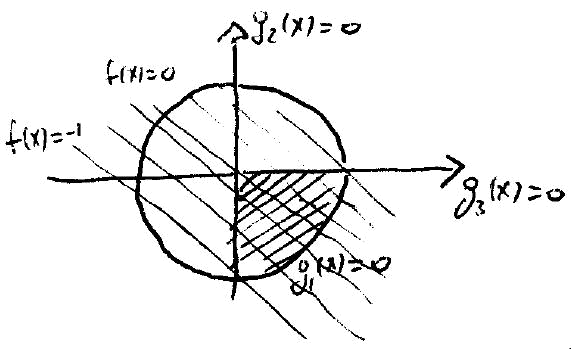
\includegraphics[width=0.4\textwidth]{imgs/ottvinc01.png}
\end{center}

Il punto di minimo (globale) \`e $\overline{x}=(0, -1)$, mentre
$\nabla f(\overline{x}) =
\begin{pmatrix}
 1 \\
 1
\end{pmatrix}
$
$$
T(X, \overline{x} ) \subseteq \{d \in \mathbb{R}^{n} \; | \; \underbracket{d_1 + d_2}_{\nabla f(\overline{x})^{T}d} \geq 0 \}
 $$
\begin{center}
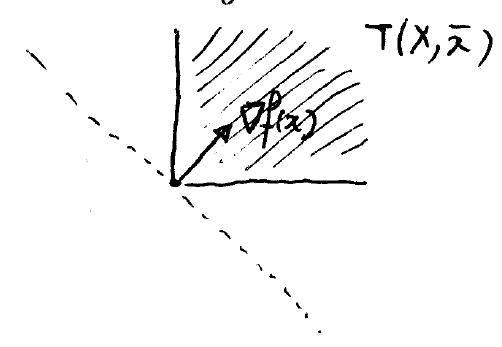
\includegraphics[width=0.4\textwidth]{imgs/ottvinc03.png}
\quad
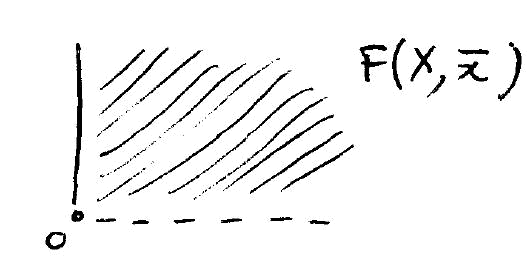
\includegraphics[width=0.4\textwidth]{imgs/ottvinc04.png}
\end{center}
Notiamo che nel cono tangente \`e presente la semiretta orizzontale,
che \`e invece assente nel cono delle direzioni ammissibili: questo \`e
dovuto al fatto che nel cono delle direzioni ammissibili siamo costretti
a fissare un $d$, e non riusciamo quindi ad arrivare alla semiretta orizzontale.
Ci riusciamo invece avendo una sottosuccessione $d_n$ che tende a $d$, dove
$d$ in questo caso \`e ancora la semiretta orizzontale. \\
Vincoli attivi: $g_1, g_2$
$$\overline{x} = (0,1)$$
$$ g_1(\overline{x}) = 0 \qquad
 g_2(\overline{x}) = 0 \qquad
 g_3(\overline{x}) = -1 < 0 $$
Calcoliamo i gradienti
$$ \nabla g_1(\overline{x}) =
\begin{pmatrix}
0 \\
-2
\end{pmatrix}\quad \nabla g_2(\overline{x})=
\begin{pmatrix}
-1 \\
 0
\end{pmatrix}
$$
\begin{center}
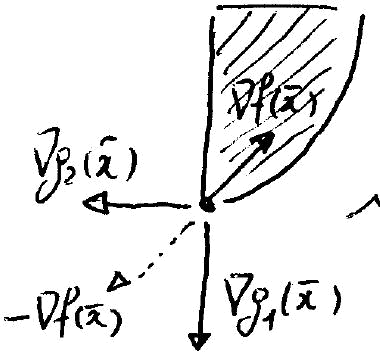
\includegraphics[width=0.25\textwidth]{imgs/ottvinc02.png}
\end{center}

Abbiamo che $-\nabla f(x)$ appartiene al cono tangente
 $\{\nabla g_1(\overline{x}),\nabla g_2(\overline{x})\}$
ed \`e combinazione lineare di $\nabla g_1$ e $\nabla g_2$.
Assomiglia al simplesso.
$$ - \nabla f(\overline{x}) = \lambda_1 \nabla g_1(\overline{x}) +
\lambda_2 \nabla g_2(\overline{x}) $$
\end{example}
Cerchiamo di formalizzare matematicamente questo concetto.
Dobbiamo sfruttare la rappresentazione di $X$.
$$ X  = \{x \in \mathbb{R}^{n} \; | \; g_i(x) \leq 0 , i = 1 \ldots n \}
\quad g_i: \mathbb{R}^{n} \rightarrow \mathbb{R} \text{ diff. }
$$
Supponiamo esplicitamente che $X$ sia espressa in questa forma,
Poi introdurremo le uguaglianze. \\
Sostituiamo le formule con il loro sviluppo al prim'ordine.
I  vincoli non attivi \`e come se non ci fossero: consideremo i
vincoli attivi.
\paragraph{Linearizzazioni di $X$ in $\overline{x} \in X$}

$$I(x) = \{ i \; | \; g_i(\overline{x}) = 0 \}
\quad \text{ indici dei vincoli attivi in } \overline{x}
$$

$$ g_i(x) \approx \cancel{\underbrace{g_i(\overline{x})}_{\text{se attivo}}} + \nabla g_i(\overline{x})^{T}(\underbracket{x-\overline{x}}_{d})$$
Andiamo quindi a inserire in $L$ le approssimazioni al primo
ordine delle $g_i$ che sono vincoli attivi.
$$L_{<}(X, \overline{x}) = \{ d \in \mathbb{R}^{n} \; | \;
\nabla g_i(\overline{x})^{T}d < 0, i \in I(\overline{x}) \} \text{ (APERTO) } $$
$$L_{\leq}(X, \overline{x}) = \{ d \in \mathbb{R}^{n} \; | \;
\nabla g_i(\overline{x})^{T}d \leq 0, i \in I(\overline{x}) \} \text{ (CHIUSO) } $$

\begin{proposition}
  Sia $\overline{x} \in X $.
 Allora
 $$L_{<} (X, \overline{x}) \subseteq T(X, \overline{x})
 \subseteq L_{\leq}(X, \overline{x}) $$
\begin{todo}
Qui manca la dimostrazione che sarebbe bene includere.
\end{todo}
\end{proposition}
Abbiamo quindi inscatolato il cono tangente.
\begin{example}[Continuazione esempio precedente]
Vediamo nell'esempio le linearizzazioni.
$$ L_{<}(X, \overline{x}) = \{ d \in \mathbb{R}^{2} \; | \;
-2 d_2 < 0, - d_1 < 0 \}  = int\; \mathbb{R}^{2}_{+}$$
$$ L_{\leq}(X, \overline{x}) = \{ d \in \mathbb{R}^{2} \; | \;
-2 d_2 \leq 0, - d_1 \leq 0 \}  =  \mathbb{R}^{2}_{+}$$
Abbiamo quindi che
$$ L_{\leq}(X, \overline{x}) = T(X, \overline{x})$$
$L_{<}(X, \overline{x})$ \`e un insieme aperto mentre $T(X, \overline{x})$ \`e un insieme chiuso,
l'unico caso in cui possono coincidere \`e che i 2 insiemi sono aperti e
chiusi: questo avviene quando tali insiemi sono tutto lo spazio, questo
corrisponde a non avere vincoli attivi. \\
Se $\overline{x}$ \`e un punto interno alla regione ammissibile,
il cono tangente \`e tutto $\mathbb{R}^{n}$, perch\'e ci possiamo
avvicinare da ogni direzione.
\`E possibile che $T$ e $L_{\leq}$ siano diversi, ossia
$$ T(X, \overline{x}) \subsetneq L_{\leq}(X, \overline{x})$$
Ad esempio (verificare per casa)
$$ X = \{ x \in \mathbb{R}^{2} \; | \; x_1^{2} - x_2^{2} \leq 0 \}
\quad \overline{x} = (0,0)
$$
\end{example}
La diversit\`a tra $T(X, \overline{x}) $ e $L_{\leq}(X, \overline{x})$ \`e quella che ci da fastidio.
Vogliamo riscrivere la condizione
$$ \nabla f(\overline{x})^{T} d \geq 0 \quad
\forall d \in T(X, \overline{x}) $$
Utilizzeremo $L_{<}$, grazie infatti all'inclusione
$L_{<}(X, \overline{x}) \subseteq T(X, \overline{x})$ abbiamo:
$$
\nabla f(\overline{x})^{T} d \geq 0 \quad
\forall d \in T(X, \overline{x})
\quad \Longrightarrow \quad
\left\lbrace d ~| \; \left\{
\begin{array}{l}
\nabla f(\overline{x})^{T} d < 0 \\
 \nabla  g_i(\overline{x})^{T} d < 0 \quad \forall i \in I(\overline{x})
\end{array}
\right.
\right\rbrace
= \emptyset
$$
ossia il sistema non ammette alcuna soluzione
$d \in \mathbb{R}^{n}$.
Possiamo dimenticare il cono tangente: abbiamo una condizione
necessaria di ottimalit\`a fatta esclusivamente dalla funzione
obiettivo e dai vincoli. Il teorema che andremo ad enunciare,
risultato dell'algebra lineare, ci fornisce un sistema \emph{duale},
che ammette soluzione quando il sistema di partenza non ne ha, 
e viceversa.

\begin{theo}[Motzkin]

Siano $a_k, b_i, c_j \in \mathbb{R}^{n}$  con $k \in I^{<}, i \in I^{\leq},
j \in  I^{=}$, con $I^{<}, I^{\leq}, I^{=}$ insiemi
finiti di indici con $I^{<} \neq \emptyset$. Allora

$$
\begin{array}{l}
\left\{
\begin{array}{l}
a_k^{T}d < 0, k \in I^{<} \\
b_i^{T}d \leq 0, i \in I^{\leq} \\
c_j^{T}d = 0, j \in I^{=} \\
\end{array}
\right. \\
\text{ non ha soluzione } d \in \mathbb{R}^{n}
\end{array}
\Longleftrightarrow
\begin{array}{l}
\left\{
\begin{array}{l}
\displaystyle \sum_{k \in I^{<}} \theta_k a_k + \displaystyle \sum_{i \in I^{\leq}}
 v_i b_i + \displaystyle \sum_{j \in I^{=}} \mu_j c_j = 0 \\
\theta_k \geq 0 , v_{i} \geq 0 , \mu_{j} \in \mathbb{R}
\end{array}
\right.  \\
\text{ ammette soluzione in cui i } \theta_k \text{ non sono tutti nulli}
\end{array}
$$
\end{theo}

Quindi, applicando questo teorema in versione di Gordan al sistema $(5)$ con $\overline{x}$
punto di minimo locale di $(P)$, e quindi $(5)$ non ammette soluzione, si ottiene che:
$$
\left\{
\begin{array}{l}
\nabla f(\overline{x})^{T} d < 0 \\
 \nabla  g_i(\overline{x})^{T} d < 0 \quad \forall i \in I(\overline{x})
\end{array}
\right.
= \emptyset
\quad
\xLongleftrightarrow{\text{ con } I^{\leq} = \emptyset, I^{=} = \emptyset}
\quad
\begin{array}{c}
\exists \theta \geq 0, \lambda_i \geq 0 \text{ con } i \in I(\overline{x})
\text{ non tutti nulli tali che } \\
\theta \nabla f(\overline{x}) +
\displaystyle \sum_{i \in I(\overline{x})} \lambda_i \nabla g_i(\overline{x})
 = 0
\end{array}
$$

Ponendo
$$\lambda_i = 0 \; \forall i \notin I(\overline{x}) $$
Otteniamo
$$
\left\{
\begin{array}{l}
\theta \nabla f(\overline{x}) + \displaystyle \sum_{i=1}^{n}
\lambda_i \nabla g_i(\overline{x}) = 0  \\
\lambda_i g_i(\overline{x}) = 0 \quad i = 1 \ldots n
\end{array}
\right.
$$

Abbiamo quindi una nuova riformulazione del teorema
\begin{theo}[Fritz John]
Sia $\overline{x}$ un punto di minimo locale di (P). Allora
$\exists \theta \geq 0, \lambda_i \geq 0$ con $i=1, \ldots, n$
non tutti nulli (sia $\theta$ che $\lambda_i$ ) tali che
$$
(FJ)
\left[
\begin{array}{ll}
\theta \nabla f(\overline{x}) + \displaystyle \sum_{i=1}^{n}
\lambda_i \nabla g_i(\overline{x}) = 0 & (FJ_1)
\\
\lambda_i g_i(\overline{x}) =0 \quad i=1 \ldots n & (FJ_2)
\end{array}
\right.
$$
\end{theo}
Il vincolo $(FJ_2)$ esprime una condizione di complementarit\`a:
nel caso che il vincolo sia attivo in $\overline{x}$ (cioé $g_{i}(\overline{x}) = 0$) può essere $\lambda_i \geq 0$. Altrimenti se il vincolo non è attivo ($g(\overline{x}) < 0$) deve essere $\lambda_i = 0$.

Per la verifica di ottimalità di $\overline{x}$ siamo passati da un controllo di infiniti vettori alla risoluzione di un sistema di equazioni che \`e trattabile. Risolvendo il sistema di Fritz--John si otterranno $\theta$ e dei $\lambda_i$. Questi ultimi varranno $0$ per i vincoli non attivi, fornendo un'indicazione su quali siano i vincoli che effettivamente entrano in gioco nella risoluzione del problema di minimizzazione. I $\lambda_i$ vengono chiamati \emph{moltiplicatori di Lagrange}.

Che fastidio ci da $\theta =0$ ? Compaiono esclusivamente i vincoli
del problema, non c'\`e la funzione obiettivo: vorremo che le condizioni
valessero per $\theta \neq 0$. \\
Se le condizioni di Fritz John valgono con $\theta =0$, allora
$\{ \nabla g_i(\overline{x}) \}_{i \in I(\overline{x})}$ sono linearmente dipendenti.\\
Allora aggiungiamo la negazione come ipotesi. Otteniamo una
nuova versione del teorema.
\begin{observation}
$$(FJ) \text{ valgono con } \theta = 0 \quad \Longrightarrow \quad
\{ \nabla g_i(\overline{x})\}_{i \in I(\overline{x})} \text{ linearmente dipendenti}
$$
\end{observation}
\begin{theo}[Karush-Kuhn-Tucker]
Sia $\overline{x}$ un punto di minimo locale di (P) e supponiamo
che $\{\nabla g_i(\overline{x})\}_{i \in I(\overline{x})}$ siano linearmente
indipendenti. Allora
$\exists  \lambda_i \geq 0$ con $i=1, \ldots, n$ tali che
$$
\begin{array}{ll}
(KKT_1) & \nabla f(\overline{x}) + \displaystyle \sum_{i=1}^{n}
\lambda_i \nabla g_i(\overline{x}) = 0
 \\
(KKT_2) &  \lambda_i g_i(\overline{x}) = 0 \quad i =1 \ldots n
\end{array}
$$
\end{theo}
Le condizioni di ottimalit\`a KKT sono costituite dal sistema di equazioni
e disequazioni (non lineari):
$$
\left\{
\begin{array}{llll}
(KKT_1) & \nabla f(\overline{x}) + \displaystyle \sum_{i=1}^{n}
\lambda_i \nabla g_i(\overline{x}) = 0 & &  \text{(Ottimalit\`a)}

 \\
(KKT_2) &  \lambda_i g_i(\overline{x}) = 0 &  i =1 \ldots n
& \text{(Complementarit\`a)}
 \\
 \\
(KKT_3) &  g_i(x) \leq 0  & i=1 \ldots n 
 & \text{(Ammissibilit\`a (1) )} \\
 \\
(KKT_4) &   \lambda_i \geq 0   & i=1 \ldots n
& \text{(Ammissibilit\`a (2) )}
\end{array}
\right.
$$
dove $(KKT_3)$ e $(KKT_4)$ sono le condizioni di ammissibilit\`a,
nelle incognite $x \in \mathbb{R}^{n}, \lambda = (\lambda_1, \ldots, \lambda_n) \in \mathbb{R}^{n}$

\begin{notes}
Le condizioni di complementarit\`a fanno in modo che il moltiplicatore
di Lagrange associato ad un vincolo possa essere strettamente
maggiore di 0 solamente nel caso in cui il vincolo \`e attivo, infatti:
\\
\\
\textbf{Caso 1} 
$$
\left\{
\begin{array}{l}
 \underbracket{\lambda_i}_{\geq 0} g_i(\overline{x}) = 0  \\
 g_i(x) = 0
\end{array}
\right.
$$
\vspace{0.5cm}
\textbf{Caso 2} 
$$
\left\{
\begin{array}{l}
 \underbracket{\lambda_i}_{=0} g_i(\overline{x}) = 0  \\
 g_i(x) < 0
\end{array}
\right.
$$

\end{notes}
\begin{observation}[I moltiplicatori di Lagrange sono unici]
Infatti se $\overline{\lambda} = (\overline{\lambda}_1, \ldots, \overline{\lambda}_{n})$
e $\hat{\lambda} = (\hat{\lambda_1}, \ldots, \hat{\lambda}_{n})$
soddisfano $(KKT_1)$, sottraendo un sistema di equazioni dall'altro
si ottiene:
$$ \displaystyle \sum_{i \in I(\overline{x})}
  ( \overline{\lambda}_{i} - \hat{\lambda}_{i}) \nabla g_i(\overline{x}) = 0
$$
Allora
$\overline{\lambda}_{i} = \hat{\lambda}_{i} \quad \forall i \in [1 \ldots n]$
a causa della lineare indipendenza dei gradienti.
\end{observation}
Qualifiche dei vincoli: $\equiv$ condizioni su vincoli per cui (FJ) valgono
 con $\theta = 1$. Altre qualifiche sono:

 \begin{defn}[Condizioni di Slater]
   \begin{enumerate}
   \item    $g_i$  convesse per ogni $i \in I (\overline{x})$
   \item $\exists \hat{x} \in \mathbb{R}^{n} \text{ t.c. } g_i(\hat{x}) < 0
         \quad i = 1 \ldots n$
   \end{enumerate}
 \end{defn}

 \begin{defn}[Condizioni di Mangasarian-Fromovits]
   $\exists d \in \mathbb{R}^{n}:  \nabla g_i(\hat{x})^{T}d < 0
   \text{ per ogni } i \in I(\overline{x})$
   (cio\`e $ L_{<} (X, \hat{x}) \neq \emptyset$)
 \end{defn}

Lineare indipendenza si pu\`o sostituire con una delle due
condizioni

\begin{example}
\`E importante notare che le condizioni $(KKT)$ non possono sempre essere utilizzate per dimostrare che un punto è di minimo locale. In questo esempio troveremo un punto di minimo in cui non valgono le ipotesi del teorema $KKT$\\
$n=2, m=2$
$$ f(x) = x_1 + x_2^{2} $$
$$ g_1(x) = x_1^{2} + (x_2 -1)^{2} -1 \qquad
 g_2(x) = x_1^{2} + (x_2+1)^{2} -1 $$
 \begin{center}
   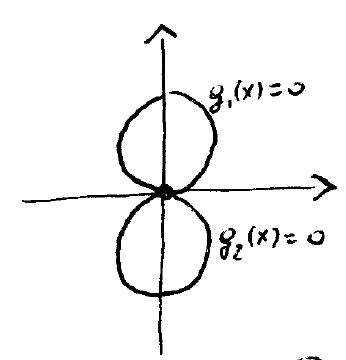
\includegraphics[width=0.25\textwidth]{imgs/ottvinc05.png}
 \end{center}
La regione ammissibile \`e data da un solo punto:
$$
X = \left\{
\begin{pmatrix}
0 \\
0
\end{pmatrix}
\right\}
$$
Di conseguenza il punto di minimo può essere soltanto:
$$
\overline{x} =
\begin{pmatrix}
0 \\
0
\end{pmatrix}
\quad \Longrightarrow \quad 
I(\overline{x}) = \{1, 2 \}
$$

Calcolo dei gradienti:
$$
\nabla f(\overline{x}) =
\begin{pmatrix}
1 \\
0
\end{pmatrix}
\quad
\nabla g_1(\overline{x}) =
\begin{pmatrix}
2 \overline{x}_1 \\
2(\overline{x}_2 -1)
\end{pmatrix}
=
\begin{pmatrix}
0 \\
-2
\end{pmatrix}
\quad
\nabla g_2(\overline{x}) =
\begin{pmatrix}
2 \overline{x}_1 \\
2(\overline{x}_2 + 1)
\end{pmatrix}
=
\begin{pmatrix}
0 \\
2
\end{pmatrix}
$$
Calcolo delle condizioni KKT: entrambi i vincoli sono attivi.
$$
\begin{pmatrix}
1 \\
0
\end{pmatrix}
+
\lambda_1
\begin{pmatrix}
0 \\
-2
\end{pmatrix}
+ \lambda_2
\begin{pmatrix}
0 \\
2
\end{pmatrix}
=
\begin{pmatrix}
1 \\
2(\lambda_2 - \lambda_1)
\end{pmatrix} =
\begin{pmatrix}
0 \\
0
\end{pmatrix}
$$
\begin{itemize}
\item Il sistema sopra non ha soluzione, quindi il teorema $(KKT)$ non si può applicare in $\overline{x}$. Questa condizione si verifica perché non sono verificate le ipotesi di $(KKT)$, dato che $\nabla g_1(\overline{x})$ e $\nabla g_2(\overline{x})$ non sono linearmente indipendenti:
$$
\begin{pmatrix}0 \\2 \end{pmatrix}
=
-1 \cdot
\begin{pmatrix}0 \\-2\end{pmatrix}
$$

\item le condizioni $(FJ)$ valgono con  per 
$\theta = 0 \quad \lambda_2 = \lambda_1 > 0$
\item Le qualifiche dei vincoli non valgono:
$$
\left\{
  \begin{array}{l}
  \nabla g_1(\overline{x}), \nabla g_2 (\overline{x}) \quad \text{ linearmente dipendenti} \\
L_{<}(X, \overline{x}) = \emptyset  
  \end{array}
\right.
$$
\end{itemize}
Il cono tangente \`e pi\`u piccolo del linearizzato.
\end{example}

\paragraph{Vincoli lineari}
Esistono dei casi in cui le qualifiche dei vincoli non servono, \`e
il caso dei vincoli lineari.
I vincoli lineari non richiedono alcuna qualificazione affinch\`e
valgano le condizioni $KKT$. \\
I vincoli lineari sono della forma
$$ X = \{ x \in \mathbb{R}^{n} \; | \; Ax \leq b \} \quad
A \in \mathbb{R}^{m \times n}, b \in \mathbb{R}^{n} $$

\begin{proposition}
Sia $\overline{x} \in X$, allora 
$$T(X, \overline{x}) =L_{\leq} (X, \overline{x})$$
\end{proposition}
\begin{notes}
No dimostrazione, ma sulla note c'e'.
\end{notes}
\paragraph{Condizioni KKT nella programmazione lineare}
Consideriamo la programmazione lineare
$$ \max \{c^{T}x \; | \;  Ax \leq b \}  = - \min\{(-c)^{T}x \; | \; Ax \leq b \}$$
Sappiamo che valgono le condizioni $KKT$ sempre. \\
Come minimo
$$  -\min \{(-c)^{T}x \; | \; x \in X \} $$
Obiettivo
$$ f(x)  = -c^{T}x \quad \nabla f(\overline{x}) = - c $$
Vincoli
$$ g_i(x) = A_i x - b_i  \quad \rightarrow \quad \nabla g_i(x) = A_i$$
Condizioni moltiplicatori di Lagrange 
$$ -c + \displaystyle \sum_{i=1}^{n} \lambda_i A_i
= -c + \lambda^{T} A = 0
$$
Ossia
$$
\begin{array}{ll}
   \lambda^{T}A = c  & (KKT_1) \text{ (ammisibilit\`a duale 1) } \\
  \lambda \geq 0  & (KKT_4) \text{ (ammissibilit\`a duale 2) } \\
   Ax \leq b & \text (KKT_3) \text{ (ammissibilit\`a primale)} \\
\lambda_i \underbracket{(b_i - a_i^{T}x)}_{g_i} = 0 &
 (KKT_2) \text{ (scarti complementari) } 
\end{array}
$$

\subsubsection{Caso con introduzione di vincoli di uguaglianza}
Consideriamo adesso il caso in cui $X$ sia descritto tramite
vincoli di disuguaglianza ed uguaglianza.
$$(P) \quad \min\{ f(x) : x \in X \} \quad
X = \{ x \in \mathbb{R}^{n} \; | \; g_i(x) \leq 0, h_j(x) = 0
\; i=1\ldots n, j =1 \ldots p
\}
$$
con
$$ g_i: \mathbb{R}^{n} \rightarrow \mathbb{R}, i=1, \ldots n \; , \;
h_j :  \mathbb{R}^{n} \rightarrow \mathbb{R}, j=1,\ldots p 
 \text{ differenziabili}
$$
\begin{notes}
La tentazione sarebbe di ragionare nel metodo pi\`u semplice possibile:
$$
 h_j(x) = 0 \equiv
\left\{
\begin{array}{l}
h_j(x) \leq 0 \\
- h_j(x) \leq 0
\end{array}
\right.
$$
ossia considerare un vincolo di uguaglianza come due disuguaglianze.
Ma in questo caso si avrebbe
$$
L_{<}(X, \overline{x}) = \{d \in \mathbb{R}^n ~|~ \nabla g_i(\overline{x})^Td <0 \quad i \in I(\overline{x})\} = \emptyset
$$

Quindi dal punto di vista matematico l'equivalenza sopra è corretta, ma noi siamo interessati a trovare un metodo per la verifica dell'ottimalità linearizzando i vincoli e utilizzando $L_<$, quindi per i nostri fini dobbiamo procedere diversamente.
\end{notes}

$$L_{\leq} =
\{ d \in \mathbb{R}^{n} \; | \; \nabla g_i(\overline{x})^{T} d \leq 0
\quad i \in I(\overline{x}),\quad \nabla h_j(\overline{x})^{T}d = 0
\quad j=1 \ldots p \}
$$
Lo riportiamo a $L_{<}$
$$L_{<} =
\{ d \in \mathbb{R}^{n} \; | \; \nabla g_i(\overline{x})^{T} d < 0
\quad i \in I(\overline{x}), \quad \nabla h_j(\overline{x})^{T}d = 0
\quad j=1 \ldots p \}
$$
L'inclusione 
$$T(X, \overline{x}) \subseteq L_{\leq}(X, \overline{x})$$
si dimostra similmente al caso delle sole disuguaglianze
mentre l'inclusione 
$$ L_{<}(X, \overline{x}) \subseteq T(X, \overline{x})$$
richiede l'ipotesi che $\{ \nabla h_j(\overline{x})\}_{j=1\ldots p}$
siano linearmente indipendenti. \\
A questo punto ripercorriamo la teoria:

$$
\begin{array}{l}
 \nabla f(\overline{x})^{T} d \geq 0\quad
\forall d \in T(X, \overline{x})   \\
\{ \nabla h_j(\overline{x})\}_{j=1\ldots p} \text{ linearmente
indipendenti}
\end{array}
\quad
\Longrightarrow_{L_{<} \subseteq T}
\quad
\begin{array}{l}
\left\{
\begin{array}{l}
  \nabla f(\overline{x})^{T}d < 0  \\
 \nabla g_i(\overline{x})^{T}d < 0 \quad i \in I(\overline{x}) \\
 \nabla h_j(\overline{x})^{T}d = 0 \quad j =1 \ldots p \\
\end{array}
\right. \\
\text{Non ammette soluzione } d \in \mathbb{R}^{n}
\end{array}
$$
Possiamo applicare il teorema di Motzkin, ottenendo le condizioni
di Fritz John, e imponendo la qualifica otteniamo le condizioni KKT.
\begin{theo}[Karush-Kuhn-Tucker con vincoli di uguaglianza e disuguaglianza]
Sia $\overline{x} \in X $ un punto di minimo locale di $(P)$ e supponiamo
che i vettori $\{ \nabla g_i(\overline{x})\}_{i \in I(\overline{x})} 
\cup
\{ \nabla h_j(\overline{x}) \}_{j=1\ldots p}
$
siano linearmente indipendenti. Allora esistono $\lambda_i \geq 0$
con $i=1\ldots n$,  $\mu_{j} \in \mathbb{R}$ con $j=1\ldots p$ tali che
$$
\begin{array}{ll}
\nabla f(\overline{x}) +
\displaystyle  \sum_{i=1}^{n} \lambda_i \nabla g_i (\overline{x})
+ \displaystyle \sum_{j=1}^{p} \mu_j \nabla h_j(\overline{x}) = 0 & 
(\overline{KKT}_1) \text{ Moltiplicatori di Lagrange }    \\
\lambda_i g_i(\overline{x})=0 \quad i =1 \ldots n &
(\overline{KKT}_2) \text{ Complementarit\`a}
\end{array}
$$
\end{theo}
Le condizioni di ottimalit\`a $\overline{KKT}$ sono quindi costituite dal sistema
di equazioni e disequazioni (non lineari):
$$
\left\{
\begin{array}{lll}
\nabla f(\overline{x}) +
\displaystyle  \sum_{i=1}^{n} \lambda_i \nabla g_i (\overline{x})
+ \displaystyle \sum_{j=1}^{p} \mu_j \nabla h_j(\overline{x}) = 0 & & 
(\overline{KKT}_1) \text{ Moltiplicatori di Lagrange }    \\
\lambda_i g_i(\overline{x})=0 & i =1 \ldots n &
(\overline{KKT}_2) \text{ Complementarit\`a} \\
g_i(x) \leq 0 & i=1\ldots n & (\overline{KKT}_3)  \text{ Ammissibilit\`a (1) } \\
h_j(x) = 0 & j=1\ldots p  & (\overline{KKT}_5)  \text{ Ammissibilit\`a (2) } \\
\lambda_i \geq 0 & i=1\ldots n  & (\overline{KKT}_4)  \text{ Ammissibilit\`a (3) }
\end{array}
\right.
$$
nelle incognite $x \in \mathbb{R}^{n}, \lambda = (\lambda_1, \ldots, \lambda_n) \in \mathbb{R}^{n}, \mu = (\mu_1, \ldots, \mu_p) \in \mathbb{R}^{p}$

\begin{defn}[Funzione Lagrangiana]
  $$ L(x, \lambda, \mu) = f(x) + \displaystyle \sum_{i=1}^{n} \lambda_i
g_i(x) + \displaystyle \sum_{j=1}^{p} \mu_j h_j(x)$$
si dice \emph{funzione Lagrangiana} di
$$ (P) \quad  \min\{f(x): \; g_i(x)\leq 0, i=1\ldots n, \;
h_j(x)=0, j=1\ldots p \}
$$
\end{defn}

\begin{observation}
$$(\overline{KKT}_1) \equiv \nabla_x L(x, \lambda, \mu) = 0$$

Nota che il grandiente \`e calcolato solamente per la variabile $x$.
\end{observation}
\paragraph{Altre qualifiche dei vincoli}

 \subparagraph{Slater}
 \begin{itemize}
 \item $h_j: \text{ affini }: h_j(x) = a_j^{T}x + b_j, \quad j=1\ldots p $
 \item $g_i: \text{ convesse per ogni  }: i \in I(\overline{x})$
 \item $\{\nabla h_j(\overline{x})\}_{j=1\ldots p }$ linearmente indipendenti
 \item $\exists \hat{x} \in \mathbb{R}^{n}$ tale che
 $ 
\left\{
  \begin{array}{ll}
  g_i(\hat{x})< 0 & i=1\ldots n \\
  h_j(\hat{x}) = 0 & j=1\ldots p
   \end{array}
\right.
$
 \end{itemize}
 \subparagraph{Mangasarian-Fromovitz}
 \begin{itemize}
 \item $\{ \nabla h_j(\overline{x})\}_{j=1\ldots p}$ linearmente indipendenti
 \item $\exists d \in \mathbb{R}^{n}$ tale che
$  
\left\{
 \begin{array}{ll}
  \nabla g_i(\overline{x})^{T}d \leq 0 & i \in I(\overline{x})  \\
  \nabla h_j(\overline{x})^{T}d = 0 & j=1\ldots p  
 \end{array}
(\Longleftrightarrow L_{<}(X, \overline{x}) \neq \emptyset)
\right.
$
 \end{itemize}

\begin{exercise}
  Possiamo provare a scrivere le condizioni KKT per il problema
  duale
  $$ \min \{ b^{T}\lambda \; | \; \lambda \in X \} $$
  $$ X = \{ \lambda \in \mathbb{R}^{n} \; | \; \lambda^{T}A = c,
  \lambda \geq 0 \}$$
Indicazione, deve venire fuori $\lambda_i(A_ix - b_i) = 0 \quad
i=1 \ldots n$
\end{exercise}
\begin{exercise}
 $$g_i(x) \leq 0
\Longleftrightarrow g_i(x) = s_i^{2} = 0
 $$
Trasformiamo il problema in soli vincoli di uguaglianza con le slack
$(x,s) \in \mathbb{R}^{n+m} $
Scrivere le condizioni KKT in questo caso.
Problema: per le ugaglianze serve la lineare indipendenza.
\end{exercise}
%% Questo non mi è chiaro...io toglierei
%% NIC

Le condizioni KKT sono necessarie per l'ottimalit\`a, 
ma per $f$ convessa vale il seguente teorema:
\begin{theo}
Siano $f$ e $g_i$ convesse con $i \in I(\overline{x})$ per
qualche $\overline{x} \in X$ e siano
$h_j$ affini con $j=1\ldots p$ ($h_j(x) = a_j^{T}x- b_j$
per opportuni $a_j \in \mathbb{R}^{n}, b_j \in \mathbb{R}$).
Se esistono $\lambda_i \geq 0$, con $i=1\ldots n$ e
$\mu_j \in \mathbb{R}$ con $j=1\ldots p$, tali che
valgono $(KKT_1)$ e $(KKT_2)$ allora $\overline{x}$
\`e un punto di minimo globale.
\end{theo}

\section{Metodi per la risoluzione}
\subsection{Eliminazione di variabili}
\begin{example}
Vogliamo minimizzare la norma, che \`e una funzione convessa.
  $$ \min \{ x_1^{2} + x_2^{2} \} \qquad x_1 + x_2 -1 = 0$$
Una strada possibile \`e usare i moltiplicatori KKT e trovare
la soluzione. \\
In realt\`a alcune variabili possono essere espresse da altre
$$ x_2 = 1 - x_1 $$
Sostituendo nella funzione obiettivo
$$ \min \{ x_1^{2} + (1-x_1)^{2} \; | \; x_1 \in \mathbb{R} \} $$
Abbiamo eliminato una variabile: \`e diventato un problema
di ottimizzazione non vincolata: lo possiamo risolvere con
i metodi dell'ottimizzazione non vincolata.

Il gradiente \`e
$$ 2x_1 - 2(1 -x_1) = 0 \quad \Rightarrow \quad x_1 = \frac{1}{2}$$
\end{example}
\begin{exercise}
 Provare a risolvere il problema con le condizioni KKT.
\end{exercise}
Saremmo tentati ad usare sempre questa strada, ma non \`e sempre possibile

\begin{example}
  $$ \min \{ x_1^{2} + x_2^{2} \;  \} \qquad  x_2^{2} - (x_1-1)^{3} = 0  $$
 $$ x_2^{2} = (x_1-1)^{3} $$
 $$ \min\{ x_1^{2} + (x_1 -1)^{3} \; | \; x_1 \in \mathbb{R} \} $$
 $x_1 \rightarrow - \infty$
Inferiormente illimatato, ma non \`e possibile!
Cosa abbiamo sbagliato?
Il vincolo

$$
x_2^{2} = (x_1  - 1)^{3}
$$
Sta nascondendo il vincolo $x_1 \geq 1$.
\end{example}
L'eliminazione di variabili funziona bene solamente nel caso
di vincoli lineari.

\begin{example}
  $$ \min\{ f(x) \; | \; Ax = b  \}
\quad A \in \mathbb{R}^{m \times n} \quad m \leq n \quad
A \text{ rango massimo}
$$
Se una matrice $A$ ha rango massimo, si possono riordinare le $n$ colonne
delle matrice $A$ in modo che le prime $m$ siano linearmente indipendenti

$$ A = [ \underbracket{A_1}_{m \times m}  \; | \underbracket{A_2}_{m \times n-m} ]$$
$$x =
\begin{pmatrix}
x^{1} \\
x^{2}
\end{pmatrix}
x^{1} \in \mathbb{R}^{m} \quad x^{2} \in \mathbb{R}^{n}
$$

$$x^{1} = A_1^{-1}(b -A_2 x^{2})
\quad
\Longleftrightarrow
A_1 x^{1} = b -A_2 x^{2}
\quad
\Longleftrightarrow
Ax = b
$$
Problemi: abbiamo una matrice da invertire, potremmo soffrire
di problemi di condizionamento, cancellazione, per questo
queste tecniche non vengono molto utilizzate.

\end{example}
Accenno ad un'altra tecnica
\begin{example}
  $$ \min \{ x_1^{2} + x_2^{2} \; | \; x_1 + x_2 -1 = 0 \}$$
  Possiamo penalizzare la funzione obiettivo nei punti
  in cui $x$ non soddisfa i vincoli.
  In questo esempio potremmo usare come funzione obiettivo
$$ x_1^{2}  + x_2^{2} + r(x_1 + x_2 -1)^{2} $$
Nuova famiglia di problemi
$$
\min \{ x_1^{2} + x_2^{2} + r(x_1 + x_2 -1 ) \; | \; x_1, x_2 \in \mathbb{R} \}
$$
\end{example}
%\begin{exercise}
%  Provare a risolvere il problema per $r$ fissato.
%\end{exercise}


% Bigi 24 Maggio
\subsection{Excursus di metodi sull'ottimizzazione vincolata}
\paragraph{Condizioni KKT nel caso disuguaglianze e uguaglianze}

$$
\nabla f(x) +
\displaystyle \sum_{i=1}^{n}
\lambda_i \nabla g_i(x) +
\displaystyle \sum_{j=1}^{p}
\mu_j \nabla h_j(x) = 0
\Longleftrightarrow
\nabla_x L(x, \lambda,\mu)=0
$$

$$
\begin{array}{l}
\lambda_i g_i(x) = 0 \quad i=1\ldots n \\
 g_i(x) \leq 0 \quad i=1\ldots n  \\
 h_j(x) = 0 \quad j=1 \ldots p  \\
 \lambda_i \geq 0 \quad i = 1 \ldots r
\end{array}
$$

\paragraph{Lagrangiana}
$$
L(x, \lambda, \mu) = f(x) +
\displaystyle \sum_{i=1}^{n}
\lambda_i g_i(x) +
\displaystyle \sum_{j=1}^{p}
\mu_j h_j(x)
$$

$$ (P) \quad  \min\{f(x): \; g_i(x)\leq 0, i=1\ldots n, \;
h_j(x)=0, j=1\ldots p \}
$$

\subsubsection{Trasformazione di problemi in forma non vincolata:
penalizzazione esterna}

\paragraph{Esempio introduttivo}
Consideriamo la minimizzazione della seguente funzione obiettivo convessa:
$$
\min \{ x_1^{2} + x_2^{2} : x_1 + x_2 -1 =0 \}
$$
e insieriamo una forma di penalizzazione, portando il vincolo
nella funzione con un coefficiente $r$ di penalizzazione:
$$
\min \{ x_1^{2} + x_2^{2} + r(x_1 + x_2 -1)^{2} \; : \;
x \in \mathbb{R}^{2}
\}
$$
$r$ indica di quanto penalizziamo, quando siamo al di fuori
della regione ammissibile: il fatto che ci sia un'espressione
al quadrato \`e voluto, in modo che la cosa funzioni sia
per quantit\`a negative che positive.
Vogliamo capire la relazione che c'\`e fra $r$ (parametro
di penalizzazione) ed il problema originale.
La funzione \`e convessa, minimo locale implica minimo
globale.
Deriviamo, le due equazioni sono
$$\text{Derivata rispetto a } x_1 \; :\;  2x_1 + 2r(x_1 + x_2 -1) = 0 $$
$$ \text{Derivata rispetto a }x_2\; : \; 2x_2 + 2r(x_1 + x_2 -1) = 0$$
Indichiamo con $x^{r}$ il punto di minimo.
$$ x_1^{r} = x_2^{r} = \dfrac{r}{1+2r}$$
Cosa succede per $r \to \infty$?
Il limite \`e $\dfrac{1}{2}$. \\
Scriviamo le condizioni KKT che in questo danno una condizione
necessaria \`e sufficiente all'ottimalit\`a.
$$
\left\{
\begin{array}{ll}
 2 x_1 + \mu = 0  & \\
 2 x_2 + \mu = 0  & \\
 x_1 + x_2 = 1 & \text{Ammissibilit\`a}
\end{array}
\right.
$$
Otteniamo
$$ x_1^{*} = x_2^{*} = \dfrac{1}{2}
\qquad \mu = -1
$$
Proviamo a porci in una situazione pi\`u generale: sia $h$ il
vincolo di uguaglianza.
$$
\min \{f(x) + rh^2(x) \; | \; x \in \mathbb{R}^{n} \}
$$
e deriviamo rispetto a $x$
$$\nabla f(x^{r}) + \underbrace{2rh(x^{r})}_{\mu} \nabla h(x^{r})
$$
dove $x^r$ \`e il minimo: abbiamo ottenuto un moltiplicatore

$$ 2r(x_1^{r} + x_2^{r} -1 ) = \dfrac{-2r}{1+2r}
\xrightarrow{r \to + \infty} = -1
$$
Quindi, almeno in questo caso, portare $r$ ad infinito corrisponde
a risolvere il problema originale.
\paragraph{Teoria della penalizzazione}
Consideriamo il problema generico con vincoli di uguaglianza e di disuglianza. Introduciamo la \emph{Funzione di penalizzazione} $p_r$ che tiene conto di entrambi i tipi di vincoli e utilizziamo un parametro $r > 0$:
$$ p_r(x) = f(x) + r \cdot \left(
\displaystyle \sum_{i=1}^{n} ({g^+_i})^{2}(x) +
\displaystyle \sum_{j=1}^{p} h_j^{2}(x)
\right)
$$
dove $g^+_i$ deve ancora essere definita. Come abbiamo visto, per i vincoli di uguaglianza è corretto moltiplicare $r$ per $h_j^2(h)$, ma per quanto riguarda le disuguaglianze non possiamo comportarci allo stesso modo (ovvero prendere $g^+_i = g_i$ dato che in questo modo penalizzeremmo anche le soluzioni che si discostano dai vincoli verso l'interno della regione ammissibile.

Prendendo invece
$$ g_i^{+}(x) = \max\{ 0, g_i(x) \} $$
la penalizzazione $g_i^{+}(x)$ vale $0$ se il vincolo è rispettato, $>0$ altrimenti.

Si pone dunque un nuovo problema di minimizzazione:
$$(P_r) \quad \min \{ p_r(x) : x \in \mathbb{R}^{n}  \} $$

\begin{notes}
$g_i^+(x)$ non \`e necessariamente differenziabile, ma elevandola al quadrato lo diventa. Tuttavia,  non \`e differenziabile due volte, quindi per minimizzare $p_r(x)$ non possiamo applicare il metodo di Newton che usa le derivate seconde.\end{notes}


\paragraph{Osservazioni preliminari}
$$x \in X \quad \Rightarrow \quad p_r(x) = f(x) $$
$$x \notin X \quad \Rightarrow \quad p_r(x) > f(x) $$
Quindi in generale
$$ p_r(x) \geq f(x) \quad \forall x \in \mathbb{R}^{n}, ~ \forall r \geq 0$$
Chiamamo $\overline{v}$ il valore ottimo del problema originale $(P)$
e $\overline{v}_r$ l'ottimo del problema con la penalizzazione $(P_r)$,
i valori in generale non coincidono!

\begin{observation}
$\overline{v} = \min\{f(x) ~:~ x \in X\} \geq \min\{p_r(x) ~:~ x \in \mathbb{R}^{n} \} = \overline{v}_r \quad \forall ~ r \geq 0$. Quindi $$\overline{v} \geq
sup\{ \overline{v}_{r}\; : \; r \geq 0 \}$$
Inoltre $r_1 \geq r_2 \; \Rightarrow \; \overline{v}_{r_1}
\geq \overline{v}_{r_2}$ (cioé $\min\{p_r(x)\}$ è non decrescente all'aumentare di $r$) e quindi
$$sup\{\overline{v}_{r}\; : \;r \geq 0 \} = \lim_{r \to \infty} 
\overline{v}_r $$
\end{observation}

\begin{proposition}
  Supponiamo che $x_r$ sia un punto di minimo
 \emph{globale} di $(P_r)$.
Ogni punto di accumulazione di $\{x^r\}_r$ \`e
un punto di minimo globale di $(P)$.
\end{proposition}
\begin{observation}
$x^{r}$ ammissibile, cio\`e $x^{r} \in X \Rightarrow x^{r}$ punto
di minimo globale di $(P)$. Infatti
$$ \overline{v} \geq \overline{v}_{r} = p_{r}(x^k) 
\underbracket{=}_{x^{k} \in X}  f(x^{k})$$ da cui
$\overline{v} = f(x^{k})$ poich\'e $x^{k}$ \`e ammissibile.
\end{observation}
Quindi in genere $\{x^{k} \}$ \`e costituita da punti
non ammissibili, cio\`e ``esterni'' alla regione
ammissibile $X$ (da cui il nome di \emph{penalizzazione esterna}.
Dovremo accontentarci di una soluzione approssimata.\\
Sappiamo che:
$$ x^{k} \text{ punto di minimo globale di } (P_r) \quad
\Rightarrow \quad \nabla p_r(x^{r}) = 0 $$
Calcoliamo esplicitamente il gradiente:
$$
\begin{array}{l}
0 =  \nabla p_r(x^{k}) = 
\nabla f(x^{k}) +
\displaystyle \sum_{i=1}^{n} 2r_k g_i^{+}(x^{k})
\nabla g_i^{+}(x^{k}) + \displaystyle \sum_{j=1}^{p} 2r_k h_j(x^{k})
\nabla h_j(x^{k})
\end{array}
$$
$$ \lambda_i^{k} =  2r_{k}g_i^{+}(x^{k}) \; i=1\ldots m
\qquad  \text{e} \qquad
\mu_j^{k} = 2r_{k}h_j(x^k) \; j=1\ldots p$$
 sono i moltiplcatori associati
a $x^{k}$ per il problema $(P)$ \\
 (Attenzione, le altri condizioni
KKT, cio\`e ammisiblit\`a e complementarit\`a in genere
non sono soddisfatte $[g_i^{+}(x^{k}) > 0 \Rightarrow \lambda_i^{k} > 0 ]$
)
\begin{theo}
Supponiamo che $f, g_i, h_j$ siano differenziabili
con continuit\`a. Siano
$r_k \uparrow + \infty, \tau_k \downarrow 0$ e
$x^{k} \in \mathbb{R}^{n}$ un punto tale che
$||\nabla p_{r_k}(x^{k})||_{2} \leq \tau_k$.
Allora ogni punto di accumulazione $x^{*}$ di
$\{x^{k}\}$ tale che
$$
\{ \nabla h_j(x^{*}) \}_{j=1\ldots p}  \cup
\{ \nabla g_i(x^{*}) \}_{i \in I(\overline{x})}
\quad \text{linearmente indipendenti}
$$
soddisfa le condizioni
KKT per $(P)$ con i moltiplicatori
$$ \lambda_i^{*}, \mu_j^{*}$$
dati da
$$
\begin{array}{ll}
\displaystyle \lambda_i^{*} = \lim_{l \to + \infty}
2r_{{k}_l} g^{+}_i(x^{k_l})  &  i =1 \ldots n \\
\displaystyle \mu_{j}^{*} = \lim_{l \to + \infty} 2r_{k_{l}}
h_j(x^{k_l}) & j =1 \ldots p
\end{array}
 $$
dove $\{x^{k_l}\}$ \`e una sottosuccessione tale che
$x^{k_l} \rightarrow x^{*} $
\end{theo}

\begin{observation}[Problema mal condizionato]
Fare tendere $r$ a $ + \infty$ pu\`o portare a dei seri
problemi di malcondizionamento:
$\nabla_r^{2}$ pu\`o risultare mal condizionato per $r$ grande.
Prendiamo il problema visto nell' esempio iniziale :
$$ Pr(x) = x_1^{2} + x_2^{2} + r(x_1 + x_2 -1)^{2} $$
$$ \nabla_{r}^{2} p_r(x) =
\begin{pmatrix}
2(1+r) & 2r \\
2r &  2(1+r)
\end{pmatrix}
$$

Gli autovalori $\lambda_1^{r} = 2$
, $\lambda_2^{r} = 2(1+2r)$. \\
Gli autovettori corrispondenti sono
$\begin{pmatrix}
1 \\
-1
\end{pmatrix}
$
,
$\begin{pmatrix}
 1 \\
-1
\end{pmatrix}
$,
ma $\lambda_2^{r} \xrightarrow{ r \to \infty} +\infty$
\end{observation}

\subsubsection{Metodo dei moltiplicatori}
Funziona solo con vincoli di uguaglianza, ma basta
introdurre le variabili di slack $s_i$, dette anche
variabili di scarto,  per le disugliaglianza, ossia
$$ g_i(x) \leq 0 \quad \longrightarrow  \quad g_i(x) + s_i^{2} = 0$$
Consideriamo il problema
$$ (P_{eq}) \quad \min\{ f(x) \; : \; h_j(x) = 0 \; j=1\ldots p \} \quad
(f,h \; \text{differenziabili con continuit\`a}) $$

Supponiamo di perturbare i vincoli di uguaglianza $h_j(x)$ di una
quantit\`a $\delta_j$, a questo punto la funzione di penalizzazione
esterna diventa:
$$f(x) + r
\displaystyle \sum_{j=1}^{p}
\left[h_j(x) - \delta_j\right]^{2} =
f(x) + \displaystyle
\sum_{j=1}^{p}
\underbracket{(-2r\delta_j)}_{\mu_j}h_j(x) +
r \displaystyle
\sum_{j=1}^{p}
h_j^{2}(x) +
\underbracket{r \displaystyle \sum_{j=1}^{p} \delta_j^{2}}_{costante}
$$
Abbiamo ottenuto la Lagrangiana aumentata (dalla penalizzazione)
\begin{defn}[Lagrangiana aumentata per $(P_{eq})$]
$$L_r(x, \mu) = f(x)+ \displaystyle  \sum_{j=1}^{p}
\mu_j h_j(x) + r \displaystyle \sum_{j=1}^{p}
h_j^{2}(x)
$$  
\end{defn}
Adesso abbiamo qualcosa in pi\`u con cui giocare: i moltiplicatori.
Nella precedente funzione obiettivo non erano presenti.
Supponiamo che $\overline{x}$ e $\overline{\mu}$ soddisfino
le condizioni KKT. In questo caso si ottiene che $\overline{x}$ \`e
un punto stazionario della Lagrangiana aumentata vista come funzione
della sola $x$ dove i moltipicatori sono fissati.

\begin{observation}
$L_r(\cdot, \mu)$ \`e la funzione di penalizzazione esterna di
$$ (PL_{eq}(\mu))\quad \min\{ f(x) + \displaystyle \sum_{j=1}^{p}
\mu_j h_j(x) \; : \; h_j(x) = 0\; j=1\ldots p\}
$$
dove $\mu \in \mathbb{R}^{p}$ \`e fissato, mentre $L_r$ \`e
la funzione lagrangiana di 
$$(P_{eq}(r))\quad \min\{ f(x) + r \displaystyle \sum_{j=1}^{p}
h_j^{2}(x) \; : \;   h_j(x) = 0\; j=1\ldots p \}
$$
dove $r>0$ \`e fissato. Sia $(PL_{eq}(\mu))$ che $(P_{eq}(r))$ sono
problemi equivalenti a $(P_{eq})$, in quanto gli addendi
della penalizzazione, quando ci si trova all'interno della
regione ammissibile, si annullano.
\end{observation}

\begin{theo}
Se $\overline{x} \in \mathbb{R}^{n},
\overline{\mu}\in \mathbb{R}^{p}$
soddisfano le condizioni di KKT per ($P_{eq}$), allora
$\overline{x}$ \`e un punto stazionario di $ L_r(\cdot, \overline{\mu})$
\end{theo}
\begin{thproof}
  $$
\nabla_x L_r (\overline{x}, \overline{\mu}) =
 \nabla f(\overline{x}) + \displaystyle \sum_{j=1}^{p}
\overline{\mu}_{j} \nabla h_j(\overline{x}) 
+ 2r \displaystyle \sum_{j}^{p} h_j(\overline{x}) \nabla h_j(\overline{x})
\underbracket{=}_{KKT \Rightarrow h_j(\overline{x})=0} 
\nabla f(\overline{x}) + \displaystyle \sum_{j=1}^{p}
\overline{\mu}_j \nabla h_j(\overline{x})
\underbracket{=}_{(\overline{KKT_1})} 0
$$
\end{thproof}
Questo risultato non \`e in genere vero per la funzione esterna.
\begin{center}
 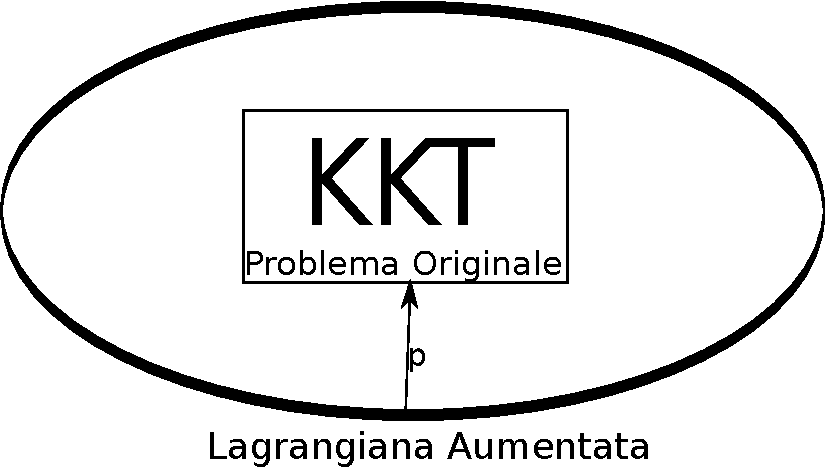
\includegraphics[width=0.35\textwidth]{imgs/lagrangianaaumentata.pdf}
\end{center}
In parole povere un punto stazionario del problema della langrangiana
aumentata \`e candidato ad essere un punto
che rispetta che condizioni KKT del problema originario e, per $p \to \infty$,
il cerchio, che per l'appunto contiene i punti stazionari
della lagrangiana aumentata,  tende a restringersi: \`e questa
l'idea che sta alla base del algoritmo che vedremo fra poco.
\begin{proposition}
 Siano $r_k \uparrow + \infty$ (successione che va a infinito)
, $\{ \mu^{k} \}_{k}$ successione limitata e 
supponiamo che 
$$
 (P_{eq}(x^{k})) \quad \min \{ L_{r}(x, \mu^{k}) \; : \; x \in \mathbb{R}^{n} \}
$$
ammetta un punto di minimo globale $x^{k}$ per ogni $k$.
Allora ogni punto di accumulazione di $\{x^{k}\}_{k}$ \`e
un punto di minimo globale di $(P_{eq})$.
%Allora ogni punto di accumulazione della successione
%$x^{k}$ \`e un punto di minimo globale del problema
%$(P_e)$, quello con i soli vincoli di uguaglianza.
\end{proposition}

\begin{observation}
Calcoliamo il gradiente della Lagrangiana aumentata
 $$
 \nabla_{x} L_{r}(x, \mu) = 
 \nabla f(x) + \displaystyle \sum_{j=1}^{p}
 \underline{(\mu_j + 2rh_j(x))}
 \nabla h_j(x)
 $$
\end{observation}
Questa osservazione ci suggerisce una tecnica per
aggiornare i moltiplicatori


\begin{theo}
Siano $\{ \mu^{k} \} \subseteq \mathbb{R}^{p} $ limitata,
$r_k \uparrow + \infty$, $\tau_k \downarrow 0$ e
$x^{k} \in \mathbb{R}^{n}$ tale che $|| \nabla L_{r_{x}}(x^{k}, \mu^{k})||_{2}
\leq \tau_{k} $.
Allora ogni punto di accumulazione $x^{*}$ di $\{ x^{k} \} $ tale che
$\{ \nabla h_j(x^{*})\}_{j=1\ldots p }$ siano  linearmente indipendenti
soddisfa le condizioni KKT insieme ai moltiplicatori
$$\mu_j^{*} = \displaystyle \lim_{l \to \infty} (\mu_j^{k_l} +
 2 r_{k_{l}} h_j(x^{k_l})) $$
dove $\{ x^{k_l}\}$ \`e una (qualsiasi) sottosuccessione per cui
$x^{k_l} \xrightarrow{l \to + \infty} x^{*}$
\end{theo}
\paragraph{Metodo dei moltiplicatori}
\begin{center}
\fbox
{
	\begin{minipage}[position]{0.85\textwidth}
\begin{enumerate}
\item Scegliamo $\delta \in (0,1), \beta > 1,
r_0 > 0, \mu^{0} \in \mathbb{R}^{p},$ porre
$viol= + \infty; k =0$
\item Calcolare  $x^{k}\in argmin\{ L_{r_k}(x, \mu^{k}):
x\in \mathbb{R}^{n} \}$
\item Se $viol(x^{k}) = \displaystyle \max_{j=1\ldots p}  |h_j(x^{k})|  = 0$
  allora STOP, $(x^{k}, \mu^k) $ soddisfano KKT
\item 
  Se $viol(x^{k})> \delta viol$ allora
  il parametro di penalizzazione va aumentato
  \begin{equation}
    \label{eq:bigipenalest01}
 r_{k+1} = \beta r_k \quad \mu^{k+1} = \mu^{k}     
  \end{equation}
Altrimenti
$$r_{k+1}  = r_k \quad \text{ e } \quad
\mu_j^{k+1} = \mu_j^{k} +
2r_k h_j(x^k) , j =1 \ldots p$$
\item $viol = viol(x^{k}), k = k+1$ e ritornare a 2
\end{enumerate}
\end{minipage}
}
\end{center}

\begin{observation}
 Se $viol(x^{k}) = 0$ (cio\`e $x^{k}$ ammissibile, allora
$\nabla_{x} L_{r_x}(x^{k}, \mu_k) = 0 (\approx 0)$ garantisce
che $x^{k}$ e $\mu^{k}$ soddisfino le condizioni KKT per
$(P_{eq})$
\end{observation}
\begin{observation}
 L'aggiornamento (\ref{eq:bigipenalest01}) pu\`o verificarsi al pi\`u un numero
finito di volte consecutive se la condizione di stop
viene approssimata da $viol(x^{k})\leq \varepsilon$ per qualche
tolleranza $\varepsilon > 0 $ (altrimenti si avrebbe $\mu^{k}
\approx \text{cost}$ definitivamente, ma $x^{k}$ non convergerebbe
ad una soluzione ammissibile come garantito dai risultati
 precedenti). 
\end{observation}
In linea di principio anche qua si pu\`o andare a
$+ \infty$ ma avremo una buona approssimazione
dei moltiplicatori.


%% Bigi 27 Maggio

\subsubsection{Penalizzazione interna: metodi barriera}
Vediamo un altro metodo per la soluzione di problemi con vincoli non (necessariamente) convessi.

$$
\begin{array}{c}
(P_{in})\quad \min \{f(x) : x \in X \} \quad X = \{x \in \mathbb{R}^{n} :
g_i(x) \leq 0 \quad i = 1 \ldots n \} \\
 f,g_i: \mathbb{R}^{n} \rightarrow \mathbb{R}  \text{ differenziabili con continuit\`a }
\end{array}
$$

Risolviamo dunque solamente problemi in cui $X$ è formato da vincoli di disuguaglianza. Ci muoviamo inoltre sotto due ipotesi:

\begin{enumerate}
\item
 $X^{0}= \{ x \in \mathbb{R}^{n}: g_i(x) < 0 \quad i = 1 \ldots n \}
\neq \emptyset$

\item $\forall x \in X ~ \forall  \varepsilon > 0
\quad \exists y \in X^{0} \text{ tale che } ||x - y||_2 \leq \varepsilon$
\end{enumerate}
Le idee alla base della penalizzazione interna sono due:
\begin{itemize}
 \item "Aprire" la regione ammissibile, ossia eliminarne il bordo.
       Come vedremo dalle figure, questa operazione non \`e sempre possibile,
       ma quando si lavora con sistemi di vincoli, abbiamo la garanzia
       che questa operazione si possa fare senza particolari problemi
 \begin{center}
    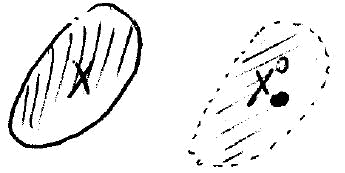
\includegraphics[width=0.25\textwidth]{imgs/ottvinc06.png}
  \end{center}
  Nel caso della figura qui sopra, sulla parte sinistra abbiamo un chiuso,
  che pu\`o essere aperto.
  \begin{center}
    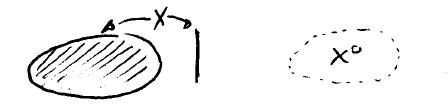
\includegraphics[width=0.35\textwidth]{imgs/ottvinc07.png}
  \end{center}
  In questo altro caso, la regione ammissibile \`e data da un insieme
  chiuso ed un segmento: non riusciamo a trovare un aperto che contenga
  tutti i punti senza introdurre nuovi punti della regione ammissibile.
 
 \item Dobbiamo introdurre una funzione obiettivo modificata, 
   che faccia schizzare a $+\infty$ il valore della funzione obiettivo
   ai bordi, in modo da garantire convergenza.
  \begin{center}
    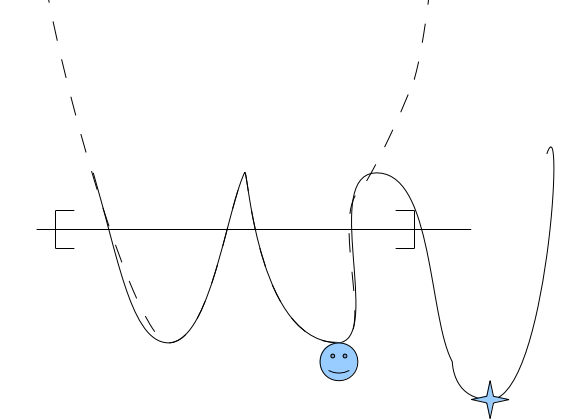
\includegraphics[width=0.45\textwidth]{imgs/penint.png}
    %%% FIXME Questa immagine è brutta e non rende per niente l'idea, andrebbe cambiata
  \end{center}
  Vediamo che il minimo globale nell'area non vincolata \`e diverso
  dal minimo globale definito nella regione ammissibile: \`e qui
  che ci viene in aiuto la funzione di penalizzazione, evidenziata
  dalla linea tratteggiata.

\end{itemize}

  Il fatto che si utilizzi un aperto e che la nuova funzione $f'(x)$ ai bordi vada a $+\infty$ ci garantisce che per trovare i punti stazionari $\overline{x}$ sia sufficiente verificare che
 $$ \nabla f'(\overline{x}) = 0$$
 Con queste due tecniche possiamo quindi utilizzare i metodi visti per l'ottimizzazione non vincolata.
 

\begin{observation}
  $ g_i$ convesse e Ipotesi $(1) \quad 
\Rightarrow \quad  Ipotesi (2)$
\end{observation}

\begin{observation}
$g_i$ continue $ \quad \Rightarrow \quad X^{0}  $ aperto
\end{observation}
L'ipotesi 2) richiede che ogni punto di $X \backslash X^{0}$ sia
il limite di una opportuna successione di punti di $X^{0}$

Ci riconduciamo ad una ottimizzazione non vincolata.
Abbiamo bisogno di una funzione, detta \emph{funzione barriera}

\begin{defn}[Funzione barriera]
Funzione definita su $X^{0}$ che tende a $+ \infty$  avvicinandosi
a punti di $X\backslash X^{0}$
$$ B:X^{0} \rightarrow \mathbb{R} \quad
B(x)\geq 0 \quad \forall x \in X^{0},
\; B(x) \to +\infty \text{ se } x \rightarrow \overline{x}
\text{ con } \overline{x} \in X\backslash X^{0}
$$
Si noti che 
$$\overline{x} \in X\backslash X^{0} ~ \Longleftrightarrow ~ \exists i \text{ t.c. } g_i(\overline{x}) = 0$$
\end{defn}

\begin{defn}[Barriera inversa]
$$ B(x) = - \displaystyle \sum_{i=1}^{n} \dfrac{1}{g_i(x)} $$
\end{defn}

\begin{defn}[Barriera logaritmica]
$$ B(x) = - \displaystyle \sum_{i=1}^{n} \log(-g_i(x)) $$
\end{defn}

\begin{observation}
In entrambi i casi: 
$$ g_i \text{ convesse } \quad \Rightarrow \quad B 
\text{ \`e convessa }$$
%(fare come esercizio:le funzioni sono monotone, 
%predere una funzione alla volta)
\end{observation}
Le funzioni barriera ci permettono di considerare, al posto del
problema di partenza
$$(PB)_{\varepsilon} \quad \min\{f(x) + \varepsilon B(x) \; : \; x \in X^{0} \} $$
La funzione barriera \`e sempre $> 0$, quindi:
$$f(x) + \varepsilon B(x) > f(x)$$
Avvicinandosi al bordo $B(x)$ tende a $+\infty$ e quindi tutto
tende a $+ \infty$.\\
Poich\'e l'insieme \`e aperto, $(PB)_{\varepsilon}$ \`e in pratica un problema di ottimizzazione non vincolata, visto che dato un punto interno a $X^0$ possiamo muoverci in qualunque direzione (con un passo di spostamento adeguato) rimanendo nella regione ammissibile. Inoltre, i punti di minimo soddisfano $\nabla(f(x) + \varepsilon B(x)) =0$
e utilizzando i metodi \emph{di discesa} visti nel Capitolo \ref{chap:ottimizzazione-non-vincolata} per risolvere i problemi di ottimizzazione non vincolata, partendo da un punto interno ad $X^0$ verrà generata una sequenza di punti apparenti ad $X^{0}$, ed anche il minimo trovato da questi metodi sarà dentro $X^0 \subset X$. Da questo deriva il nome di \emph{metodi del punto interno}.

Ma bisogna fare attenzione: è necessario partire da un punto appartente a $X^{0}$, e individuarne uno non è sempre una cosa banale (nessun vincolo deve essere attivo nel punto).
\begin{observation}
  Se $f$ e $g_i$ sono convesse anche $B(x)$ \`e convessa.
Quindi cadiamo nell'ottimizzazione convessa.
\end{observation}
Idea dei metodi: avere una successione $\varepsilon_{k}\downarrow 0
\quad x^{k} \in argmin \{ f(x) + \varepsilon_{k} B(x): x \in X^{0} \}$
utilizzando $x^{0}$ come punto iniziale. \\
Notare che la successione $x^{k}$ \`e contenuta nella regione
ammissibile $X$ (da qui il nome di \emph{penalizzazione interna}).

\begin{example}
Consideriamo il seguente problema. \\
$n=1$
$$\min \{ x : 1-x \leq 0 \}$$
$\overline{x} = 1$ \`e l'unico punto di minimo globale. \\
Proviamo ad applicare questo metodo, utilizzando la barriera
logaritmica:
$$ \min \{x - \varepsilon \log{(x-1)} : \underbracket{x > 1}_{X^{0} } 
\}$$
per $x \rightarrow 0$
il rapporto tra $x$ \`e $\varepsilon \log(x-1)$ va a $+ \infty$. \\
Calcoliamo il punto in cui il gradiente si annulla
$$\nabla (x - \varepsilon \log(x-1)) =0  \quad \Rightarrow \quad
 1- \dfrac{\varepsilon}{x-1} = 0 \quad 
\Rightarrow \quad  x = 1 + \varepsilon \; (>1)$$
Qundi la soluzione del problema barriera \`e
$$ X(\varepsilon) = 1 + \varepsilon \xrightarrow{\varepsilon \downarrow 0 } 1 $$
La funzione obiettivo in $X(\varepsilon)$ \`e
$$ X(\varepsilon) - \varepsilon \log (X(\varepsilon) -1)
= 1 + \varepsilon - \varepsilon \log \varepsilon
 $$
Pi\`u $\varepsilon$ tende a 0 pi\`u abbiamo un'esplosione.
\end{example}

\begin{example}[Esempio in due variabili]
$$
(P_{in}) \qquad
\min\{ \dfrac{1}{2} x_1^{2} +
\dfrac{1}{2} x_2^{2}  : 2 -x_1 \leq 0  \}  $$
$\overline{x}=(2,0)$ risulta essere l'unico punto di minimo
globale di $(P_{in})$: infatti le condizioni
KKT per $(P_{in})$ risultano essere
$$
 \left\{
\begin{array}{l}
\begin{pmatrix}
  x_1 \\
 x_2
\end{pmatrix}
+ \lambda
\begin{pmatrix}
  -1 \\
 0
\end{pmatrix}
=
\begin{pmatrix}
 0 \\
 0
\end{pmatrix} \\
\lambda_1(2 - x_1) = 0 \\
 x_1 \geq 2, \lambda_1 \geq 0 
\end{array}
\right.
\Rightarrow
\left\{
  \begin{array}{l}
    x_1 = \lambda_1 \\
    x_2 = 0 \\
   \lambda_1(2-x_1) = 0 \\
   x_1 \geq 2, \lambda_1 \geq 0
  \end{array}
\right.
\Rightarrow
\left\{
  \begin{array}{l}
    x_1 = \lambda_1 \\
    x_2 = 0 \\
   \lambda_1(2-x_1) = 0 \\
    \lambda_1 \geq 0
  \end{array}
\right.
\Rightarrow
\left\{
  \begin{array}{l}
    x_1 = \lambda_1  = 2\\
    x_2 = 0 
  \end{array}
\right.
$$
Cerchiamo di risolvere il problema tramite la tecnica
della barriera:
$$ (PB_{\varepsilon}) \qquad 
\min \{ \dfrac{1}{2}(x_1^{2} + x_2^{2}) - \varepsilon \log(x_1 -2) :
 x_1 > 2 \}
$$
Il punto di minimo si trova annullando il gradiente

$$
\begin{array}{l}
\begin{pmatrix}
0 \\
0
\end{pmatrix}
=
\nabla (\dfrac{1}{2}(x_1^{2} + x_2^{2}) - \varepsilon \log(x_1 -2)) = \\
\begin{pmatrix}
  x_1 - \frac{\varepsilon}{x_1 -2} \\
 x_2
\end{pmatrix}
\begin{array}{ll}
 \rightarrow x_1^{2} - 2 x_1 - \varepsilon =0 \;  \rightarrow \;
x_1 = 1 \pm \sqrt{1+ \varepsilon} \xrightarrow{x_1 > 2}
x_1 = 1 + \sqrt{1+ \varepsilon}
  \\
 \rightarrow  x_2=0
\end{array}
\end{array}
$$
$X(\varepsilon) = (1 + \sqrt{1 + \varepsilon},0)$ risulta 
essere l'unico punto di minimo globale di $(PB_{\varepsilon})$
ed inoltre $X(\varepsilon) \xrightarrow{\varepsilon \downarrow 0}(2,0)$
\end{example}
Passiamo ad una formalizzazione di quanto visto negli esempi

\begin{theo}
Ogni punto di accumulazione della successione $\{x^{k}\}$
\`e un punto di minimo globale del problema di partenza
$(P_{in})$
\end{theo}
D'ora in avanti considereremo il caso della barriera logaritmica:
$$ (PB_{\varepsilon}) \qquad \min \{ q_\varepsilon(x) = f(x) - \displaystyle \varepsilon \sum_{i=1}^{n} \log(-g_i(x)) \; : \; x \in X^{0} \}$$

Nel caso convesso ci possiamo spingere oltre.
\begin{theo}
  Supponiamo che
  \begin{itemize}
  \item  $f, g_i$ siano convesse
    \item l'insieme dei punti di minimo (globale) di $(P_{in})$ sia
      non vuoto e compatto
  \end{itemize}
  Allora:
  \begin{enumerate}
  \item La successione $\{x^{k} \}_k$ ammette almeno un punto di accumulazione
    (non stiamo parlando della regione ammissibile, stiamo usando la
    barriera)
    \item
      $f(x^{k}) \rightarrow f^{*} \quad \text{} \quad q_{\varepsilon_{k}}(x^{k})\rightarrow f^{*}, $  dove $f^{*}$ \`e il valore ottimo di $(P_{in}) $
  \end{enumerate}
\end{theo}

\paragraph{Legame con KKT}
Cosa possiamo dire sui moltiplicatori di Lagrange?
Sia $x(\varepsilon)$ \`e punto di minimo di $(PB_{\varepsilon})$.\\
Consideriamo il gradiente:
$$
\begin{array}{l}
 0 = \nabla q_{\varepsilon}(x(\varepsilon)) =
\nabla f(x(\varepsilon)) - \varepsilon
\displaystyle \sum_{i=1}^{n} \dfrac{1}{-g_i(x(\varepsilon))}
\nabla g_i(x(\varepsilon)) =  \\ 
\nabla f(x(\varepsilon)) +
\displaystyle \sum_{i}^{n} \underbracket{
\left(\dfrac{-\varepsilon}{g_i(x(\varepsilon))}\right)}_{
\footnotesize{
\begin{array}{l}
\text{moltiplicatori} \\
\text{associati a } x(\varepsilon) \\
\text{nel problema}\\
\text{originale}  (\lambda_i)
\end{array}
}
} \nabla g_i(x(\varepsilon))$$
\end{array}
$$
Sotto opportune ipotesi su un punto di minimo locale $x^{*}$
di $(P_{in})$ (tra cui la lineare indipendenza dei vettori
$\{ \nabla g_i(x^{*})\}_{i \in I(x^{*})}$ [che garantisce
l'unicit\`a dei moltiplicatori]),
\`e possibile dimostrare che:
\begin{itemize}
\item in un opportuno intorno di $x^{*}$ esiste un unico punto di
minimo locale $x(\varepsilon)$ di $(PB_{\varepsilon})$ per $\varepsilon$
sufficientemente piccolo
\item 
 $x(\varepsilon) \xrightarrow{x \downarrow 0}x^{*}$ e $
\lambda_i(\varepsilon) \xrightarrow{x \downarrow 0} \lambda_i^{*}$ sono i
moltiplicatori associati a $x^{*}$.
\end{itemize}

  
\begin{example}
Tornando all'esempio su 2 dimensioni abbiamo
$$ g_1(x) = 2 - x_1$$
e quindi
$$ \nabla_{i}(\varepsilon) =  \dfrac{-\varepsilon}{g_i(x(\varepsilon))}
= \dfrac{-\varepsilon}{\sqrt{1+\varepsilon} -1} \xrightarrow{\varepsilon \downarrow 0 }
2
$$
dove $2$ \`e il moltiplicatore di Lagrange
$\lambda_1$ associato a $x^{*}=(2,0)$.
\end{example}
%% REVIEW FROM HERE

 $x(\varepsilon)$ e $\lambda_i(\varepsilon) =  \dfrac{\varepsilon}{-g_i(x(\varepsilon))}$
soddisfano:
$$ 
\begin{array}{ll}
\nabla f(x(\varepsilon)) + \displaystyle \sum_{i=1}^{n}
\lambda_i(\varepsilon) \nabla g_i(x(\varepsilon)) = 0
& (\text{per la scelta di }\lambda_i(\varepsilon)) \\
 g_i(x(\varepsilon)) \leq 0 \quad i=1\ldots n  &
( \text{poich\'e } x(\varepsilon) \in X^{0} [\text{quindi in realt\`a } g_i(x(\varepsilon))<0 ]) \\
 \lambda_i(\varepsilon) \geq 0   &  (\text{conseguenza})
\end{array}
$$
Manca la complementarit\`a: infatti in questo caso abbiamo
$$ \lambda_i(\varepsilon) g_i(x(\varepsilon)) = - \varepsilon \neq 0 $$
ossia
$$ \lambda_i(\varepsilon)(-g_i(x(\varepsilon))) = \varepsilon > 0$$
Non \`e  rispettata la condizione di complementarit\`a: se valesse
avremmo avuto una soluzione del problema originale.
A noi interessa proprio la condizione modificata della complementarit\`a.
\paragraph{KKT approssimate}
Utilizzando le variabili di scarto (slack)
 $$
\begin{array}{ll}
\nabla f(x) + \displaystyle \sum_{i=1}^{m} \lambda_i \nabla g_i(x) = 0  & \\
 g_i(x) + s_i = 0  &    i=1 \ldots n \\
 \lambda_i s_i = \varepsilon &  i =1 \ldots n \\
  \lambda_i s_i \geq 0 \quad &  i= 1 \ldots n
\end{array}
$$

\begin{observation}
Piccola parentesi sui vincoli di uguaglianza (discorso dell'aperto):
2 possibilit\`a:
\begin{itemize}
\item Considerarli come vincoli generici
  $$ \min \{ f(x) + \varepsilon B(x) \; : \; x \in X^{0}, h_j(x) = 0 \;
  j =  1 \ldots p$$
\item Utilizzare la penalizzazione esterna
  $$ \min \{ f(x) + \varepsilon B(X) + r \displaystyle \sum_{j=1}^{p} h_j^{2}(x)
  : \; x \in X^{0} \}$$
\end{itemize}
Chiusa parentesi
\end{observation}
\paragraph{Metodi primali duali del punto interno}
Abbiamo $2m + n$ equazioni e $i$ vincoli di non negativit\`a.
Possiamo cercare di risolvere questo sistema di equazioni
adattando Newton Raphson in modo da soddisfare la condizione
$$ \lambda_i s_i \geq 0 \quad i = 1 \ldots n $$
L'idea \`e considerare $\lambda_i$ ed $s_i$ positivi
$$ \lambda_i, s_i > 0$$
La complementarit\`a non la possiamo avere, dobbiamo avere $\varepsilon >
0 $. Possiamo fare un passo nella direzione di Newton mantenendo la
positivit\`a (accorciamo il passo da unitario a qualcosa di
inferiore). Questi sono detti \emph{Metodi primali-duali del punto
interno}.  Questi metodi funzionano bene con programmazione lineare e
quadratica.  Nel caso di programmazione lineare sono quelli che hanno
rimpiazzato il simplesso. Vediamo come si pu\`o modificare il metodo
nel caso della programmazione lineare
\paragraph{Metodi primali duali per la programmazione lineare}
 $$
\begin{array}{ll}
\text{(Primale)} \quad &  \max \{c^{T}x \; : \; Ax  \leq b \} \\
 \text{(Duale)}  &  \min \{ b^{T} \lambda \; : \; A^{T}\lambda = c ,
                          \lambda \geq 0 \}
\end{array}
$$
Condizioni KKT del duale:
\begin{center}
\fbox
{
 \begin{minipage}[position]{0.75\textwidth}
$$
\begin{array}{lll}
A^{T}\lambda = c & & \text{(Ammisibilit\`a duale)}  \\
 Ax \leq b & &  \text{(Ammissibilt\`a del problema originale)} \\
 \lambda_i (b_i - a_i^{T}x) = 0 & i=1\ldots n & \\
 \lambda_i \geq 0 & i=1\ldots n  &
\end{array}
$$
\end{minipage}
}
\end{center}

Possiamo riscrivere in forma equivalente, ponendo $s=b-Ax$
$$ \overline{\text{(Primale)}} \quad   \max \{c^{T}x \; : \; Ax +s =  b \}$$

\begin{center}
\fbox
{
 \begin{minipage}[position]{0.75\textwidth}
$$
\begin{array}{lll}
A^{T}\lambda  -c = 0 & & \text{(Ammisibilit\`a duale)}  \\
 Ax +s - b = 0 & &  \text{(Ammissibilt\`a del problema originale)} \\
 \lambda_i  s_i = 0 & i=1\ldots n & \\
 \lambda_i \geq 0, s_i \geq 0 & i=1\ldots n  &
\end{array}
$$
\end{minipage}
}
\end{center}

Condizioni KKT approssimate:  sostituisce lo 0 del complementarit\`a con 
un $\varepsilon$.
\begin{center}
\fbox
{
 \begin{minipage}[position]{0.75\textwidth}
$$
\begin{array}{lll}
A^{T}\lambda  -c = 0 & & \text{(Ammisibilit\`a duale)}  \\
 Ax +s - b = 0 & &  \text{(Ammissibilt\`a del problema originale)} \\
 \lambda_i  s_i = \varepsilon & i=1\ldots n & \\
 \lambda_i \geq 0, s_i \geq 0 & i=1\ldots n  &
\end{array}
$$
\end{minipage}
}
\end{center}

Sia $F: \mathbb{R}^{n} \times \mathbb{R}^{n} \times \mathbb{R}^{n}
   \rightarrow
   \mathbb{R}^{n} \times \mathbb{R}^{n} \times \mathbb{R}^{n}$ data da
$$
F=(x, s , \lambda) =
\begin{pmatrix}
  A^{T} \lambda - c \\
  Ax  + s - b  \\
 \Lambda S e
\end{pmatrix}
$$
dove
\begin{itemize}
\item $\Lambda  = diag(\lambda_1,  \ldots , \lambda_1)$ : \ matrice diagonale con i $\lambda_i$ sulla diagonale
$$
\begin{pmatrix}
  \lambda_1 & \cdots & 0 \\
   \vdots & \ddots & \vdots \\
   0 &  \cdots & \lambda_n
\end{pmatrix}
$$
\item $S = diag(\{s_1, \ldots,  s_n \} )$
\item $e = (1, \ldots, 1)^{T} \in \mathbb{R}^{n}$
\end{itemize}
Si ha che:

$$
\text{ Condizioni KKT approssimate } \quad \Longleftrightarrow \quad
 F(x, \lambda , s) =
\begin{pmatrix}
  0 \\
 0 \\
 \varepsilon e
\end{pmatrix}\; : \; \lambda, s \geq 0
$$
Il metodo di Newton-Raphson per la risoluzione di $F(x, S, \lambda) = 0$
fornisce la direzione $d = (d_x, d_s, d_{\lambda})$ che risolve il sistema
$$(N_d) \qquad JF( x, S, \lambda) d = - F(x, S , \lambda)$$
Se $(x,s)$ \`e ammisible per $\overline{(Primale)}$ con $s_i > 0 \; i=1\ldots n$
e $\lambda$ \`e ammissibile per (Duale) con $\lambda_i > 0 \; i = 1\ldots n$,
il sistema $(N_d)$ diventa
$$
(N_d) \qquad
\begin{pmatrix}
  0 & 0 & A^{T}   \\
  A & I & 0  \\
  0 & \Lambda & S 
\end{pmatrix}
\begin{pmatrix}
d_x \\
d_{s} \\
d_{\lambda}
\end{pmatrix}
=
\begin{pmatrix}
  0 \\
  0 \\
 - \Lambda Se
\end{pmatrix}
$$

il punto corrente \`e
$$ (X, \lambda S) \rightarrow Ax +s = b \quad A^{T} \lambda_i > 0
\quad s_i > 0
$$
Affinch\'e
$
\begin{pmatrix}
  x'  \\
 s' \\
 \lambda'
\end{pmatrix}
=
\begin{pmatrix}
  x \\
 s \\
 \lambda 
\end{pmatrix}
+
\alpha
\begin{pmatrix}
  d_x \\
 d_s \\
 d_{\lambda}
\end{pmatrix}
$
soddisfi la richiesta $\lambda_i' > 0, s_i' > 0 \;
i =1 \ldots n$  \`e molto probabile che risulti
$\alpha <<1 $. \\
L''idea \`e sostiture
$ - \Lambda S e$ con $-\Lambda Se + \delta \mu e$
dove $\delta \in [0,1]$ e
$ \mu = \displaystyle \sum_{i=1}^{n} \dfrac{\lambda_i s_i}{n}$
in modo che la direzioni di Newton ``punti'' verso punti
$(x', s', \lambda ')$ per cui $\lambda_i' s_i' \approx \delta \mu > 0$.
\begin{notes}
Quello che vuole sapere che con epsilon positivo si pu\`o passare
tramite Newton-Raphson ai metodi primali duali.
\end{notes}
\paragraph{Metodo Primale Duale}
\begin{center}
\fbox
{
 \begin{minipage}[position]{0.85\textwidth}
\begin{enumerate}
\item Scegliere $(x^{0}, S^{0}, \lambda^{0})$ tale che:
   $$ Ax^{0} + s^{0} = b, \; A^{T} \lambda^{0} = c, \;
  \lambda_i^{0}>0, \; s_i^{0}>0 \quad i = 1\ldots n \; ; k=0 $$
\item Risolvere il sistema lineare:
$$
\begin{pmatrix}
 0 & 0 & A^{T} \\
 A & I & O  \\
 0 & \Lambda^{k} & S^{k}
\end{pmatrix}
\begin{pmatrix}
 d_{x}^{k} \\
 d_{s}^{k} \\
 d_{\lambda}^{k}
\end{pmatrix}
=
\begin{pmatrix}
0 \\
 0 \\
 \Lambda^{k} S^{k} e + \delta_k \mu_k e 
\end{pmatrix}
$$
dove
$$\Lambda^{k} = diag\{ \lambda_1^{k}, \ldots, \lambda_n^{k}\}, \;
S^{k} = diag\{ s_1^{k}, \ldots, s_n^{k}\}, \;
\mu^{k} = \displaystyle \sum_{i=1}^{n} \dfrac{\lambda_i^{k}s_i^{k}}{n}, \;
\delta_k \in [0,1]
$$
\item  Calcolare $\alpha^{k} > 0$ tale che
$$ s_i^{k} + \alpha_k(d_s^{k})_i, \; \lambda_i^{k} + \alpha+k(d_{\lambda})_i^{k}>0
\quad i=1 \ldots n$$
\item Porre $$(x^{k+1}, s^{k+1}, \lambda^{k+1}) = 
  (x^{k}, s^{k}, \lambda^{k}) + \alpha_k(d_x^{k}, d_s^{k}, d_{\lambda}^{k})
\quad k=k+1
$$
e ritornare a 2)
\end{enumerate}
\end{minipage}
}
\end{center}

\outbpdocument


